\appendix
% Encabezado del capítulo: "APÉNDICE" sin letra
\renewcommand*{\chapterformat}{%
  \raggedleft\MakeUppercase{\appendixname}\par\vspace{1ex}%
}
% Encabezado de página: solo "APÉNDICE"
\renewcommand{\chaptermark}[1]{\markboth{\footnotesize\MakeUppercase{\appendixname}}{}}
% Se oculta la entrada automática del índice ("A. Cálculo de ...")
\addtocontents{toc}{\protect\setcounter{tocdepth}{-1}}
\chapter{Cálculo de topologías de adyacencia e incidencia de diversos grafos}\label{apendice:topologias}
\addtocontents{toc}{\protect\setcounter{tocdepth}{\arabic{tocdepth}}}
% Entrada propia del índice: "Apéndice:" en negrita y el resto con la letra de las secciones
\addtocontents{toc}{\protect\addtokomafont{chapterentrypagenumber}{\protect\normalfont}}
\addcontentsline{toc}{chapter}{\protect\textbf{\appendixname:} \protect\normalfont Cálculo de topologías de adyacencia e incidencia de diversos grafos}
\addtocontents{toc}{\protect\setkomafont{chapterentrypagenumber}{}}


\clearpage
\begin{table}[p]
   \centering
   \footnotesize
   \renewcommand{\arraystretch}{1.15}
   \begin{tabular}{@{}>{\centering\arraybackslash}m{0.3033\textwidth}>{\centering\arraybackslash}m{0.3033\textwidth}>{\centering\arraybackslash}m{0.3033\textwidth}@{}}
      \hline
      \multicolumn{3}{@{}c@{}}{%
         \begin{tabular}{@{}>{\centering\arraybackslash}m{\dimexpr0.455\textwidth+\tabcolsep\relax}>{\centering\arraybackslash}m{\dimexpr0.455\textwidth+\tabcolsep\relax}@{}}
            $G_1$ & Matriz de adyacencia \\
            \hline
            \noalign{\vspace{6pt}}
            \rule{0pt}{0pt}$\vcenter{\hbox{\resizebox{0.25\textwidth}{!}{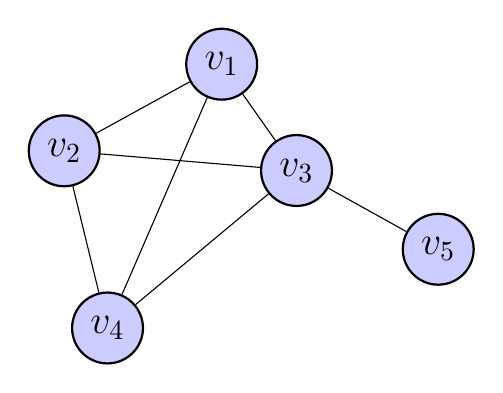
\begin{tikzpicture}[
  scale=1,
  vnode/.style={circle, fill=blue!20, draw=black, thick, minimum size=9mm, inner sep=0pt, font=\Large}
]
  % Vértices
  \node[vnode] (v1) at (2.0, 3.35) {$v_1$};
  \node[vnode] (v2) at (0.0, 2.25) {$v_2$};
  \node[vnode] (v3) at (2.95, 2.0) {$v_3$};
  \node[vnode] (v4) at (0.55, 0.0) {$v_4$};
  \node[vnode] (v5) at (4.75, 1.0) {$v_5$};

  % Aristas
  \foreach \from/\to in {v1/v2, v1/v3, v1/v4, v2/v3, v2/v4, v3/v4, v3/v5}
    \draw (\from) -- (\to);
\end{tikzpicture}
}}}$
            &
            $\vcenter{\hbox{$\displaystyle \begin{pmatrix}
         0 & 1 & 1 & 1 & 0 \\
         1 & 0 & 1 & 1 & 0 \\
         1 & 1 & 0 & 1 & 1 \\
         1 & 1 & 1 & 0 & 0 \\
         0 & 0 & 1 & 0 & 0
      \end{pmatrix}$}}$ \\
            \noalign{\vspace{6pt}}
         \end{tabular}%
      } \\
      \hline
      \multicolumn{3}{c}{\textbf{Topología de adyacencia}} \\
      \hline
      Abiertos subbásicos & Vecindades mínimas & Topología \\
      \hline
         ${A_{v_1}=\{v_2,v_3,v_4\}}$\par
         ${A_{v_2}=\{v_1,v_3,v_4\}}$\par
         ${A_{v_3}=\{v_1,v_2,v_4,v_5\}}$\par
         ${A_{v_4}=\{v_1,v_2,v_3\}}$\par
         ${A_{v_5}=\{v_3\}}$
      &
         ${U_{v_1}=\{v_1\}}$\par
         ${U_{v_2}=\{v_2\}}$\par
         ${U_{v_3}=\{v_3\}}$\par
         ${U_{v_4}=\{v_4\}}$\par
         ${U_{v_5}=\{v_1,v_2,v_4,v_5\}}$
      &
         $\{\emptyset,$ $\{v_1\},$ $\{v_2\},$ $\{v_3\},$ $\{v_4\},$ $\{v_1,v_2\},$ $\{v_1,v_3\},$ $\{v_1,v_4\},$ $\{v_2,v_3\},$ $\{v_2,v_4\},$ $\{v_3,v_4\},$ $\{v_1,v_2,v_3\},$ $\{v_1,v_2,v_4\},$ $\{v_1,v_3,v_4\},$ $\{v_2,v_3,v_4\},$ $\{v_1,v_2,v_3,v_4\},$ $\{v_1,v_2,v_4,v_5\},$ $\{v_1,v_2,v_3,v_4,v_5\}\}$ \\[6pt]
      \hline
      \multicolumn{3}{c}{\textbf{Topología de incidencia}} \\
      \hline
      Abiertos subbásicos & Vecindades mínimas & Topología \\
      \hline
         ${e_{1}=\{v_1,v_2\}}$\par
         ${e_{2}=\{v_1,v_3\}}$\par
         ${e_{3}=\{v_1,v_4\}}$\par
         ${e_{4}=\{v_2,v_3\}}$\par
         ${e_{5}=\{v_2,v_4\}}$\par
         ${e_{6}=\{v_3,v_4\}}$\par
         ${e_{7}=\{v_3,v_5\}}$
      &
         ${U_{v_1}=\{v_1\}}$\par
         ${U_{v_2}=\{v_2\}}$\par
         ${U_{v_3}=\{v_3\}}$\par
         ${U_{v_4}=\{v_4\}}$\par
         ${U_{v_5}=\{v_3,v_5\}}$
      &
         $\{\emptyset,$ $\{v_1\},$ $\{v_2\},$ $\{v_3\},$ $\{v_4\},$ $\{v_1,v_2\},$ $\{v_1,v_3\},$ $\{v_1,v_4\},$ $\{v_2,v_3\},$ $\{v_2,v_4\},$ $\{v_3,v_4\},$ $\{v_3,v_5\},$ $\{v_1,v_2,v_3\},$ $\{v_1,v_2,v_4\},$ $\{v_1,v_3,v_4\},$ $\{v_1,v_3,v_5\},$ $\{v_2,v_3,v_4\},$ $\{v_2,v_3,v_5\},$ $\{v_3,v_4,v_5\},$ $\{v_1,v_2,v_3,v_4\},$ $\{v_1,v_2,v_3,v_5\},$ $\{v_1,v_3,v_4,v_5\},$ $\{v_2,v_3,v_4,v_5\},$ $\{v_1,v_2,v_3,v_4,v_5\}\}$ \\[6pt]
      \hline
   \end{tabular}
   \caption{Topologías de adyacencia e incidencia de $G_1$}
   \label{tab:topologias_G_1}
\end{table}


\begin{table}[p]
   \centering
   \footnotesize
   \renewcommand{\arraystretch}{1.15}
   \begin{tabular}{@{}>{\centering\arraybackslash}m{0.3033\textwidth}>{\centering\arraybackslash}m{0.3033\textwidth}>{\centering\arraybackslash}m{0.3033\textwidth}@{}}
      \hline
      \multicolumn{3}{@{}c@{}}{%
         \begin{tabular}{@{}>{\centering\arraybackslash}m{\dimexpr0.455\textwidth+\tabcolsep\relax}>{\centering\arraybackslash}m{\dimexpr0.455\textwidth+\tabcolsep\relax}@{}}
            $K_{3,5}$ & Matriz de adyacencia \\
            \hline
            \noalign{\vspace{6pt}}
            \rule{0pt}{0pt}$\vcenter{\hbox{\resizebox{0.3\textwidth}{!}{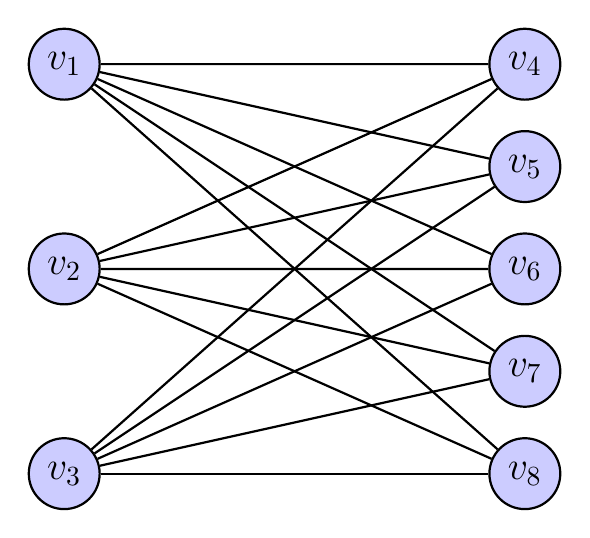
\begin{tikzpicture}[
  scale=1.3,
  vnode/.style={circle, fill=blue!20, draw=black, thick, minimum size=9mm, inner sep=0pt, font=\Large}
]
  % Partición izquierda
  \node[vnode] (v1) at (0, 4) {$v_1$};
  \node[vnode] (v2) at (0, 2) {$v_2$};
  \node[vnode] (v3) at (0, 0) {$v_3$};

  % Partición derecha
  \foreach \j in {4,...,8} {
    \node[vnode] (v\j) at (4.5, {8-\j}) {$v_{\j}$};
  }

  % Aristas: cada vértice de la izquierda con cada vértice de la derecha
  \foreach \i in {1,2,3} {
    \foreach \j in {4,...,8} {
      \draw[thick] (v\i) -- (v\j);
    }
  }
\end{tikzpicture}
}}}$
            &
            $\vcenter{\hbox{$\displaystyle \begin{pmatrix}
         0 & 0 & 0 & 1 & 1 & 1 & 1 & 1 \\
         0 & 0 & 0 & 1 & 1 & 1 & 1 & 1 \\
         0 & 0 & 0 & 1 & 1 & 1 & 1 & 1 \\
         1 & 1 & 1 & 0 & 0 & 0 & 0 & 0 \\
         1 & 1 & 1 & 0 & 0 & 0 & 0 & 0 \\
         1 & 1 & 1 & 0 & 0 & 0 & 0 & 0 \\
         1 & 1 & 1 & 0 & 0 & 0 & 0 & 0 \\
         1 & 1 & 1 & 0 & 0 & 0 & 0 & 0
      \end{pmatrix}$}}$ \\
            \noalign{\vspace{6pt}}
         \end{tabular}%
      } \\
      \hline
      \multicolumn{3}{c}{\textbf{Topología de adyacencia}} \\
      \hline
      Abiertos subbásicos & Vecindades mínimas & Topología \\
      \hline
         ${A_{v_1}=\{v_4,v_5,v_6,v_7,v_8\}}$\par
         ${A_{v_2}=\{v_4,v_5,v_6,v_7,v_8\}}$\par
         ${A_{v_3}=\{v_4,v_5,v_6,v_7,v_8\}}$\par
         ${A_{v_4}=\{v_1,v_2,v_3\}}$\par
         ${A_{v_5}=\{v_1,v_2,v_3\}}$\par
         ${A_{v_6}=\{v_1,v_2,v_3\}}$\par
         ${A_{v_7}=\{v_1,v_2,v_3\}}$\par
         ${A_{v_8}=\{v_1,v_2,v_3\}}$
      &
         ${U_{v_1}=\{v_1,v_2,v_3\}}$\par
         ${U_{v_2}=\{v_1,v_2,v_3\}}$\par
         ${U_{v_3}=\{v_1,v_2,v_3\}}$\par
         ${U_{v_4}=\{v_4,v_5,v_6,v_7,v_8\}}$\par
         ${U_{v_5}=\{v_4,v_5,v_6,v_7,v_8\}}$\par
         ${U_{v_6}=\{v_4,v_5,v_6,v_7,v_8\}}$\par
         ${U_{v_7}=\{v_4,v_5,v_6,v_7,v_8\}}$\par
         ${U_{v_8}=\{v_4,v_5,v_6,v_7,v_8\}}$
      &
         $\{\emptyset,$ $\{v_1,v_2,v_3\},$ $\{v_4,v_5,v_6,v_7,v_8\},$ $\{v_1,\allowbreak v_2,\allowbreak v_3,\allowbreak v_4,\allowbreak v_5,\allowbreak v_6,\allowbreak v_7,\allowbreak v_8\}\}$ \\[6pt]
      \hline
      \multicolumn{3}{c}{\textbf{Topología de incidencia}} \\
      \hline
      Abiertos subbásicos & Vecindades mínimas & Topología \\
      \hline
         \vspace{3pt}\begin{tabular}{@{}l@{\hspace{1.2em}}l@{}}
            ${e_{1}=\{v_1,v_4\}}$ & ${e_{9}=\{v_2,v_7\}}$ \\
            ${e_{2}=\{v_1,v_5\}}$ & ${e_{10}=\{v_2,v_8\}}$ \\
            ${e_{3}=\{v_1,v_6\}}$ & ${e_{11}=\{v_3,v_4\}}$ \\
            ${e_{4}=\{v_1,v_7\}}$ & ${e_{12}=\{v_3,v_5\}}$ \\
            ${e_{5}=\{v_1,v_8\}}$ & ${e_{13}=\{v_3,v_6\}}$ \\
            ${e_{6}=\{v_2,v_4\}}$ & ${e_{14}=\{v_3,v_7\}}$ \\
            ${e_{7}=\{v_2,v_5\}}$ & ${e_{15}=\{v_3,v_8\}}$ \\
            ${e_{8}=\{v_2,v_6\}}$ &  \\
         \end{tabular}\vspace{3pt}
      &
         \vspace{3pt}\begin{tabular}{@{}l@{\hspace{1.2em}}l@{}}
            ${U_{v_1}=\{v_1\}}$ & ${U_{v_5}=\{v_5\}}$ \\
            ${U_{v_2}=\{v_2\}}$ & ${U_{v_6}=\{v_6\}}$ \\
            ${U_{v_3}=\{v_3\}}$ & ${U_{v_7}=\{v_7\}}$ \\
            ${U_{v_4}=\{v_4\}}$ & ${U_{v_8}=\{v_8\}}$ \\
         \end{tabular}\vspace{3pt}
      &
         $\wp\left(V\left(K_{3,5}\right)\right)$ \\[6pt]
      \hline
   \end{tabular}
   \caption{Topologías de adyacencia e incidencia de $K_{3,5}$}
   \label{tab:topologias_K_35}
\end{table}

\clearpage
\begin{table}[p]
   \centering
   \footnotesize
   \renewcommand{\arraystretch}{1.15}
   \begin{tabular}{@{}>{\centering\arraybackslash}m{0.3033\textwidth}>{\centering\arraybackslash}m{0.3033\textwidth}>{\centering\arraybackslash}m{0.3033\textwidth}@{}}
      \hline
      \multicolumn{3}{@{}c@{}}{%
         \begin{tabular}{@{}>{\centering\arraybackslash}m{\dimexpr0.455\textwidth+\tabcolsep\relax}>{\centering\arraybackslash}m{\dimexpr0.455\textwidth+\tabcolsep\relax}@{}}
            3-cubo & Matriz de adyacencia \\
            \hline
            \noalign{\vspace{6pt}}
            \rule{0pt}{0pt}$\vcenter{\hbox{\resizebox{0.28\textwidth}{!}{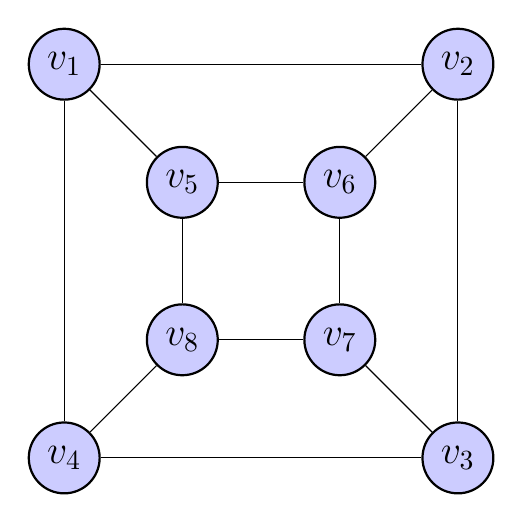
\begin{tikzpicture}[
  scale=1,
  vnode/.style={circle, fill=blue!20, draw=black, thick, minimum size=9mm, inner sep=0pt, font=\Large}
]
  % Vértices del cuadrado exterior
  \node[vnode] (v1) at (0.0, 5.0) {$v_1$};
  \node[vnode] (v2) at (5.0, 5.0) {$v_2$};
  \node[vnode] (v3) at (5.0, 0.0) {$v_3$};
  \node[vnode] (v4) at (0.0, 0.0) {$v_4$};

  % Vértices del cuadrado interior
  \node[vnode] (v5) at (1.5, 3.5) {$v_5$};
  \node[vnode] (v6) at (3.5, 3.5) {$v_6$};
  \node[vnode] (v7) at (3.5, 1.5) {$v_7$};
  \node[vnode] (v8) at (1.5, 1.5) {$v_8$};

  % Aristas
  \foreach \from/\to in {v1/v2, v2/v3, v3/v4, v4/v1,
                         v5/v6, v6/v7, v7/v8, v8/v5,
                         v1/v5, v2/v6, v3/v7, v4/v8}
    \draw (\from) -- (\to);
\end{tikzpicture}
}}}$
            &
            $\vcenter{\hbox{$\displaystyle \begin{pmatrix}
         0 & 1 & 0 & 1 & 1 & 0 & 0 & 0 \\
         1 & 0 & 1 & 0 & 0 & 1 & 0 & 0 \\
         0 & 1 & 0 & 1 & 0 & 0 & 1 & 0 \\
         1 & 0 & 1 & 0 & 0 & 0 & 0 & 1 \\
         1 & 0 & 0 & 0 & 0 & 1 & 0 & 1 \\
         0 & 1 & 0 & 0 & 1 & 0 & 1 & 0 \\
         0 & 0 & 1 & 0 & 0 & 1 & 0 & 1 \\
         0 & 0 & 0 & 1 & 1 & 0 & 1 & 0
      \end{pmatrix}$}}$ \\
            \noalign{\vspace{6pt}}
         \end{tabular}%
      } \\
      \hline
      \multicolumn{3}{c}{\textbf{Topología de adyacencia}} \\
      \hline
      Abiertos subbásicos & Vecindades mínimas & Topología \\
      \hline
         ${A_{v_1}=\{v_2,v_4,v_5\}}$\par
         ${A_{v_2}=\{v_1,v_3,v_6\}}$\par
         ${A_{v_3}=\{v_2,v_4,v_7\}}$\par
         ${A_{v_4}=\{v_1,v_3,v_8\}}$\par
         ${A_{v_5}=\{v_1,v_6,v_8\}}$\par
         ${A_{v_6}=\{v_2,v_5,v_7\}}$\par
         ${A_{v_7}=\{v_3,v_6,v_8\}}$\par
         ${A_{v_8}=\{v_4,v_5,v_7\}}$
      &
         ${U_{v_1}=\{v_1\}}$\par
         ${U_{v_2}=\{v_2\}}$\par
         ${U_{v_3}=\{v_3\}}$\par
         ${U_{v_4}=\{v_4\}}$\par
         ${U_{v_5}=\{v_5\}}$\par
         ${U_{v_6}=\{v_6\}}$\par
         ${U_{v_7}=\{v_7\}}$\par
         ${U_{v_8}=\{v_8\}}$
      &
         $\wp\left(V\left(\text{3-cubo}\right)\right)$ \\[6pt]
      \hline
      \multicolumn{3}{c}{\textbf{Topología de incidencia}} \\
      \hline
      Abiertos subbásicos & Vecindades mínimas & Topología \\
      \hline
         ${e_{1}=\{v_1,v_2\}}$\par
         ${e_{2}=\{v_1,v_4\}}$\par
         ${e_{3}=\{v_1,v_5\}}$\par
         ${e_{4}=\{v_2,v_3\}}$\par
         ${e_{5}=\{v_2,v_6\}}$\par
         ${e_{6}=\{v_3,v_4\}}$\par
         ${e_{7}=\{v_3,v_7\}}$\par
         ${e_{8}=\{v_4,v_8\}}$\par
         ${e_{9}=\{v_5,v_6\}}$\par
         ${e_{10}=\{v_5,v_8\}}$\par
         ${e_{11}=\{v_6,v_7\}}$\par
         ${e_{12}=\{v_7,v_8\}}$
      &
         ${U_{v_1}=\{v_1\}}$\par
         ${U_{v_2}=\{v_2\}}$\par
         ${U_{v_3}=\{v_3\}}$\par
         ${U_{v_4}=\{v_4\}}$\par
         ${U_{v_5}=\{v_5\}}$\par
         ${U_{v_6}=\{v_6\}}$\par
         ${U_{v_7}=\{v_7\}}$\par
         ${U_{v_8}=\{v_8\}}$
      &
         $\wp\left(V\left(\text{3-cubo}\right)\right)$ \\[6pt]
      \hline
   \end{tabular}
   \caption{Topologías de adyacencia e incidencia del 3-cubo}
   \label{tab:topologias_3_cubo}
\end{table}

\clearpage
\begin{table}[p]
   \centering
   \footnotesize
   \renewcommand{\arraystretch}{1.15}
   \begin{tabular}{@{}>{\centering\arraybackslash}m{0.3033\textwidth}>{\centering\arraybackslash}m{0.3033\textwidth}>{\centering\arraybackslash}m{0.3033\textwidth}@{}}
      \hline
      \multicolumn{3}{@{}c@{}}{%
         \begin{tabular}{@{}>{\centering\arraybackslash}m{\dimexpr0.455\textwidth+\tabcolsep\relax}>{\centering\arraybackslash}m{\dimexpr0.455\textwidth+\tabcolsep\relax}@{}}
            $R_6$ & Matriz de adyacencia \\
            \hline
            \noalign{\vspace{6pt}}
            \rule{0pt}{0pt}$\vcenter{\hbox{\resizebox{0.17\textwidth}{!}{% $R_6$ Ejemplo de retículo
% Incluido
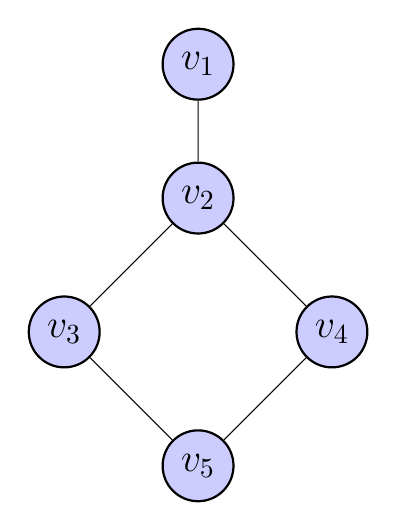
\begin{tikzpicture}[
  scale=1.7,
  vnode/.style={circle, fill=blue!20, draw=black, thick, minimum size=9mm, inner sep=0pt, font=\Large}
]
  % Vértices
  \node[vnode] (v1) at (1, 3) {$v_1$};
  \node[vnode] (v2) at (1, 2) {$v_2$};
  \node[vnode] (v3) at (0, 1) {$v_3$};
  \node[vnode] (v4) at (2, 1) {$v_4$};
  \node[vnode] (v5) at (1, 0) {$v_5$};

  % Aristas
  \foreach \from/\to in {v1/v2, v2/v3, v2/v4, v3/v5, v4/v5}
    \draw (\from) -- (\to);
\end{tikzpicture}
}}}$
            &
            $\vcenter{\hbox{$\displaystyle \begin{pmatrix}
         0 & 1 & 0 & 0 & 0 \\
         1 & 0 & 1 & 1 & 0 \\
         0 & 1 & 0 & 0 & 1 \\
         0 & 1 & 0 & 0 & 1 \\
         0 & 0 & 1 & 1 & 0
      \end{pmatrix}$}}$ \\
            \noalign{\vspace{6pt}}
         \end{tabular}%
      } \\
      \hline
      \multicolumn{3}{c}{\textbf{Topología de adyacencia}} \\
      \hline
      Abiertos subbásicos & Vecindades mínimas & Topología \\
      \hline
         ${A_{v_1}=\{v_2\}}$\par
         ${A_{v_2}=\{v_1,v_3,v_4\}}$\par
         ${A_{v_3}=\{v_2,v_5\}}$\par
         ${A_{v_4}=\{v_2,v_5\}}$\par
         ${A_{v_5}=\{v_3,v_4\}}$
      &
         ${U_{v_1}=\{v_1,v_3,v_4\}}$\par
         ${U_{v_2}=\{v_2\}}$\par
         ${U_{v_3}=\{v_3,v_4\}}$\par
         ${U_{v_4}=\{v_3,v_4\}}$\par
         ${U_{v_5}=\{v_2,v_5\}}$
      &
         $\{\emptyset,$ $\{v_2\},$ $\{v_2,v_5\},$ $\{v_3,v_4\},$ $\{v_1,v_3,v_4\},$ $\{v_2,v_3,v_4\},$ $\{v_1,v_2,v_3,v_4\},$ $\{v_2,v_3,v_4,v_5\},$ $\{v_1,v_2,v_3,v_4,v_5\}\}$ \\[6pt]
      \hline
      \multicolumn{3}{c}{\textbf{Topología de incidencia}} \\
      \hline
      Abiertos subbásicos & Vecindades mínimas & Topología \\
      \hline
         ${e_{1}=\{v_1,v_2\}}$\par
         ${e_{2}=\{v_2,v_3\}}$\par
         ${e_{3}=\{v_2,v_4\}}$\par
         ${e_{4}=\{v_3,v_5\}}$\par
         ${e_{5}=\{v_4,v_5\}}$
      &
         ${U_{v_1}=\{v_1,v_2\}}$\par
         ${U_{v_2}=\{v_2\}}$\par
         ${U_{v_3}=\{v_3\}}$\par
         ${U_{v_4}=\{v_4\}}$\par
         ${U_{v_5}=\{v_5\}}$
      &
         $\{\emptyset,$ $\{v_2\},$ $\{v_3\},$ $\{v_4\},$ $\{v_5\},$ $\{v_1,v_2\},$ $\{v_2,v_3\},$ $\{v_2,v_4\},$ $\{v_2,v_5\},$ $\{v_3,v_4\},$ $\{v_3,v_5\},$ $\{v_4,v_5\},$ $\{v_1,v_2,v_3\},$ $\{v_1,v_2,v_4\},$ $\{v_1,v_2,v_5\},$ $\{v_2,v_3,v_4\},$ $\{v_2,v_3,v_5\},$ $\{v_2,v_4,v_5\},$ $\{v_3,v_4,v_5\},$ $\{v_1,v_2,v_3,v_4\},$ $\{v_1,v_2,v_3,v_5\},$ $\{v_1,v_2,v_4,v_5\},$ $\{v_2,v_3,v_4,v_5\},$ $\{v_1,v_2,v_3,v_4,v_5\}\}$ \\[6pt]
      \hline
   \end{tabular}
   \caption{Topologías de adyacencia e incidencia de $R_6$}
   \label{tab:topologias_R_6}
   \vspace{2em}
   \begin{minipage}{\textwidth}
      \normalsize
      El grafo $R_6$ es un ejemplo de \textit{retículo}. Para información sobre la teoría de retículos puede visitarse \cite{acosta2016}. Este y los retículos que en adelante se muestren son extraídos de dicha referencia.
   \end{minipage}
\end{table}

\clearpage
\begin{table}[p]
   \centering
   \footnotesize
   \renewcommand{\arraystretch}{1.15}
   \begin{tabular}{@{}>{\centering\arraybackslash}m{0.3033\textwidth}>{\centering\arraybackslash}m{0.3033\textwidth}>{\centering\arraybackslash}m{0.3033\textwidth}@{}}
      \hline
      \multicolumn{3}{@{}c@{}}{%
         \begin{tabular}{@{}>{\centering\arraybackslash}m{\dimexpr0.455\textwidth+\tabcolsep\relax}>{\centering\arraybackslash}m{\dimexpr0.455\textwidth+\tabcolsep\relax}@{}}
            $2^3$ & Matriz de adyacencia \\
            \hline
            \noalign{\vspace{6pt}}
            \rule{0pt}{0pt}$\vcenter{\hbox{\resizebox{0.2\textwidth}{!}{% $2^3$ es ejemplo de retículo
% Incluido
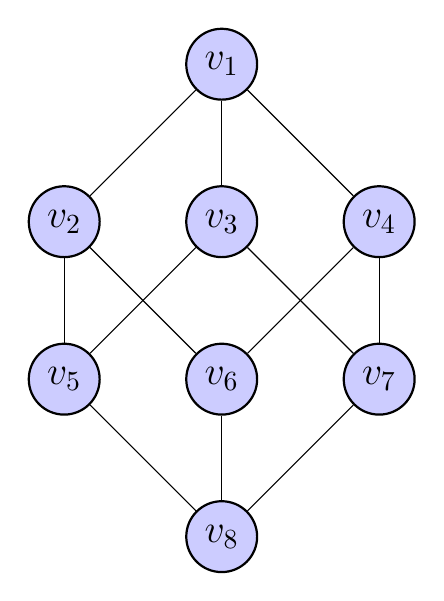
\begin{tikzpicture}[
  scale=2,
  vnode/.style={circle, fill=blue!20, draw=black, thick, minimum size=9mm, inner sep=0pt, font=\Large}
]
  % Vértices
  \node[vnode] (v1) at (1, 3) {$v_1$};
  \node[vnode] (v2) at (0, 2) {$v_2$};
  \node[vnode] (v3) at (1, 2) {$v_3$};
  \node[vnode] (v4) at (2, 2) {$v_4$};
  \node[vnode] (v5) at (0, 1) {$v_5$};
  \node[vnode] (v6) at (1, 1) {$v_6$};
  \node[vnode] (v7) at (2, 1) {$v_7$};
  \node[vnode] (v8) at (1, 0) {$v_8$};

  % Aristas
  \foreach \from/\to in {v1/v2, v1/v3, v1/v4, v2/v5, v2/v6, v3/v5,
                         v3/v7, v4/v6, v4/v7, v5/v8, v6/v8, v7/v8}
    \draw (\from) -- (\to);
\end{tikzpicture}
}}}$
            &
            $\vcenter{\hbox{$\displaystyle \begin{pmatrix}
         0 & 1 & 1 & 1 & 0 & 0 & 0 & 0 \\
         1 & 0 & 0 & 0 & 1 & 1 & 0 & 0 \\
         1 & 0 & 0 & 0 & 1 & 0 & 1 & 0 \\
         1 & 0 & 0 & 0 & 0 & 1 & 1 & 0 \\
         0 & 1 & 1 & 0 & 0 & 0 & 0 & 1 \\
         0 & 1 & 0 & 1 & 0 & 0 & 0 & 1 \\
         0 & 0 & 1 & 1 & 0 & 0 & 0 & 1 \\
         0 & 0 & 0 & 0 & 1 & 1 & 1 & 0
      \end{pmatrix}$}}$ \\
            \noalign{\vspace{6pt}}
         \end{tabular}%
      } \\
      \hline
      \multicolumn{3}{c}{\textbf{Topología de adyacencia}} \\
      \hline
      Abiertos subbásicos & Vecindades mínimas & Topología \\
      \hline
         ${A_{v_1}=\{v_2,v_3,v_4\}}$\par
         ${A_{v_2}=\{v_1,v_5,v_6\}}$\par
         ${A_{v_3}=\{v_1,v_5,v_7\}}$\par
         ${A_{v_4}=\{v_1,v_6,v_7\}}$\par
         ${A_{v_5}=\{v_2,v_3,v_8\}}$\par
         ${A_{v_6}=\{v_2,v_4,v_8\}}$\par
         ${A_{v_7}=\{v_3,v_4,v_8\}}$\par
         ${A_{v_8}=\{v_5,v_6,v_7\}}$
      &
         ${U_{v_1}=\{v_1\}}$\par
         ${U_{v_2}=\{v_2\}}$\par
         ${U_{v_3}=\{v_3\}}$\par
         ${U_{v_4}=\{v_4\}}$\par
         ${U_{v_5}=\{v_5\}}$\par
         ${U_{v_6}=\{v_6\}}$\par
         ${U_{v_7}=\{v_7\}}$\par
         ${U_{v_8}=\{v_8\}}$
      &
         $\wp\left(V\left(2^3\right)\right)$ \\[6pt]
      \hline
      \multicolumn{3}{c}{\textbf{Topología de incidencia}} \\
      \hline
      Abiertos subbásicos & Vecindades mínimas & Topología \\
      \hline
         ${e_{1}=\{v_1,v_2\}}$\par
         ${e_{2}=\{v_1,v_3\}}$\par
         ${e_{3}=\{v_1,v_4\}}$\par
         ${e_{4}=\{v_2,v_5\}}$\par
         ${e_{5}=\{v_2,v_6\}}$\par
         ${e_{6}=\{v_3,v_5\}}$\par
         ${e_{7}=\{v_3,v_7\}}$\par
         ${e_{8}=\{v_4,v_6\}}$\par
         ${e_{9}=\{v_4,v_7\}}$\par
         ${e_{10}=\{v_5,v_8\}}$\par
         ${e_{11}=\{v_6,v_8\}}$\par
         ${e_{12}=\{v_7,v_8\}}$
      &
         ${U_{v_1}=\{v_1\}}$\par
         ${U_{v_2}=\{v_2\}}$\par
         ${U_{v_3}=\{v_3\}}$\par
         ${U_{v_4}=\{v_4\}}$\par
         ${U_{v_5}=\{v_5\}}$\par
         ${U_{v_6}=\{v_6\}}$\par
         ${U_{v_7}=\{v_7\}}$\par
         ${U_{v_8}=\{v_8\}}$
      &
         $\wp\left(V\left(2^3\right)\right)$ \\[6pt]
      \hline
   \end{tabular}
   \caption{Topologías de adyacencia e incidencia de $2^3$}
   \label{tab:topologias_2_3}

   \vspace{2em}
   \begin{minipage}{\textwidth}
      \normalsize
      El grafo $2^3$ es un ejemplo de retículo.
   \end{minipage}
\end{table}

\clearpage
\begin{table}[p]
   \centering
   \footnotesize
   \renewcommand{\arraystretch}{1.15}
   \begin{tabular}{@{}>{\centering\arraybackslash}m{0.3033\textwidth}>{\centering\arraybackslash}m{0.3033\textwidth}>{\centering\arraybackslash}m{0.3033\textwidth}@{}}
      \hline
      \multicolumn{3}{@{}c@{}}{%
         \begin{tabular}{@{}>{\centering\arraybackslash}m{\dimexpr0.455\textwidth+\tabcolsep\relax}>{\centering\arraybackslash}m{\dimexpr0.455\textwidth+\tabcolsep\relax}@{}}
            $G_2$ & Matriz de adyacencia \\
            \hline
            \noalign{\vspace{6pt}}
            \rule{0pt}{0pt}$\vcenter{\hbox{\resizebox{0.2\textwidth}{!}{% Ejemplo de conjunto ordenado que no es un retículo
% Incluido
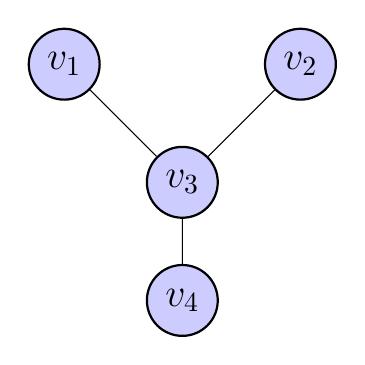
\begin{tikzpicture}[
  scale=1.5,
  vnode/.style={circle, fill=blue!20, draw=black, thick, minimum size=9mm, inner sep=0pt, font=\Large}
]
  % Vértices
  \node[vnode] (v1) at (0, 2) {$v_1$};
  \node[vnode] (v2) at (2, 2) {$v_2$};
  \node[vnode] (v3) at (1, 1) {$v_3$};
  \node[vnode] (v4) at (1, 0) {$v_4$};

  % Aristas
  \foreach \from/\to in {v1/v3, v2/v3, v3/v4}
    \draw (\from) -- (\to);
\end{tikzpicture}
}}}$
            &
            $\vcenter{\hbox{$\displaystyle \begin{pmatrix}
         0 & 0 & 1 & 0 \\
         0 & 0 & 1 & 0 \\
         1 & 1 & 0 & 1 \\
         0 & 0 & 1 & 0
      \end{pmatrix}$}}$ \\
            \noalign{\vspace{6pt}}
         \end{tabular}%
      } \\
      \hline
      \multicolumn{3}{c}{\textbf{Topología de adyacencia}} \\
      \hline
      Abiertos subbásicos & Vecindades mínimas & Topología \\
      \hline
         ${A_{v_1}=\{v_3\}}$\par
         ${A_{v_2}=\{v_3\}}$\par
         ${A_{v_3}=\{v_1,v_2,v_4\}}$\par
         ${A_{v_4}=\{v_3\}}$
      &
         ${U_{v_1}=\{v_1,v_2,v_4\}}$\par
         ${U_{v_2}=\{v_1,v_2,v_4\}}$\par
         ${U_{v_3}=\{v_3\}}$\par
         ${U_{v_4}=\{v_1,v_2,v_4\}}$
      &
         $\{\emptyset,$ $\{v_3\},$ $\{v_1,v_2,v_4\},$ $\{v_1,v_2,v_3,v_4\}\}$ \\[6pt]
      \hline
      \multicolumn{3}{c}{\textbf{Topología de incidencia}} \\
      \hline
      Abiertos subbásicos & Vecindades mínimas & Topología \\
      \hline
         ${e_{1}=\{v_1,v_3\}}$\par
         ${e_{2}=\{v_2,v_3\}}$\par
         ${e_{3}=\{v_3,v_4\}}$
      &
         ${U_{v_1}=\{v_1,v_3\}}$\par
         ${U_{v_2}=\{v_2,v_3\}}$\par
         ${U_{v_3}=\{v_3\}}$\par
         ${U_{v_4}=\{v_3,v_4\}}$
      &
         $\{\emptyset,$ $\{v_3\},$ $\{v_1,v_3\},$ $\{v_2,v_3\},$ $\{v_3,v_4\},$ $\{v_1,v_2,v_3\},$ $\{v_1,v_3,v_4\},$ $\{v_2,v_3,v_4\},$ $\{v_1,v_2,v_3,v_4\}\}$ \\[6pt]
      \hline
   \end{tabular}
   \caption{Topologías de adyacencia e incidencia de $G_2$}
   \label{tab:topologias_G_2}

   \vspace{2em}
   \begin{minipage}{\textwidth}
      \normalsize
      El grafo $G_2$ es un ejemplo de conjunto ordenado que no es un retículo. También es un ejemplo de árbol.
   \end{minipage}
\end{table}

\clearpage
\begin{table}[p]
   \centering
   \footnotesize
   \renewcommand{\arraystretch}{1.15}
   \begin{tabular}{@{}>{\centering\arraybackslash}m{0.3033\textwidth}>{\centering\arraybackslash}m{0.3033\textwidth}>{\centering\arraybackslash}m{0.3033\textwidth}@{}}
      \hline
      \multicolumn{3}{@{}c@{}}{%
         \begin{tabular}{@{}>{\centering\arraybackslash}m{\dimexpr0.455\textwidth+\tabcolsep\relax}>{\centering\arraybackslash}m{\dimexpr0.455\textwidth+\tabcolsep\relax}@{}}
            $P_9$ & Matriz de adyacencia \\
            \hline
            \noalign{\vspace{6pt}}
            \rule{0pt}{0pt}$\vcenter{\hbox{\resizebox{0.25\textwidth}{!}{% $P_9$ Ejemplo de retículo de Post
% Incluido
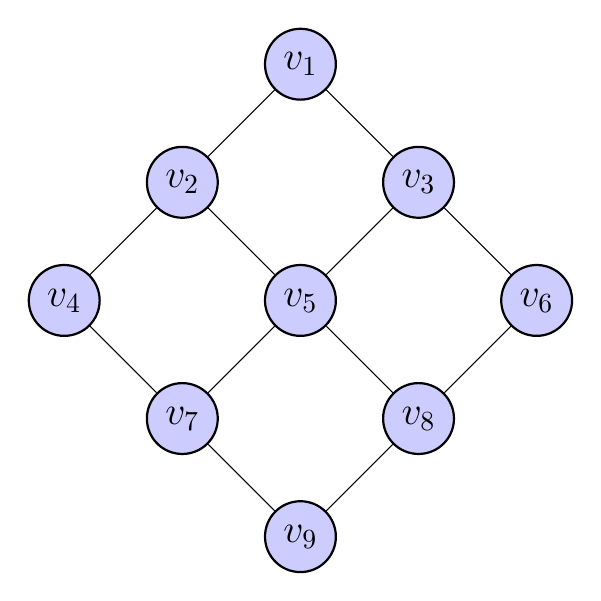
\begin{tikzpicture}[
  scale=1.5,
  vnode/.style={circle, fill=blue!20, draw=black, thick, minimum size=9mm, inner sep=0pt, font=\Large}
]
  % Vértices
  \node[vnode] (v1) at (2, 4) {$v_1$};
  \node[vnode] (v2) at (1, 3) {$v_2$};
  \node[vnode] (v3) at (3, 3) {$v_3$};
  \node[vnode] (v4) at (0, 2) {$v_4$};
  \node[vnode] (v5) at (2, 2) {$v_5$};
  \node[vnode] (v6) at (4, 2) {$v_6$};
  \node[vnode] (v7) at (1, 1) {$v_7$};
  \node[vnode] (v8) at (3, 1) {$v_8$};
  \node[vnode] (v9) at (2, 0) {$v_9$};

  % Aristas
  \foreach \from/\to in {v1/v2, v1/v3, v2/v4, v2/v5, v3/v5, v3/v6,
                         v4/v7, v5/v7, v5/v8, v6/v8, v7/v9, v8/v9}
    \draw (\from) -- (\to);
\end{tikzpicture}
}}}$
            &
            $\vcenter{\hbox{$\displaystyle \begin{pmatrix}
         0 & 1 & 1 & 0 & 0 & 0 & 0 & 0 & 0 \\
         1 & 0 & 0 & 1 & 1 & 0 & 0 & 0 & 0 \\
         1 & 0 & 0 & 0 & 1 & 1 & 0 & 0 & 0 \\
         0 & 1 & 0 & 0 & 0 & 0 & 1 & 0 & 0 \\
         0 & 1 & 1 & 0 & 0 & 0 & 1 & 1 & 0 \\
         0 & 0 & 1 & 0 & 0 & 0 & 0 & 1 & 0 \\
         0 & 0 & 0 & 1 & 1 & 0 & 0 & 0 & 1 \\
         0 & 0 & 0 & 0 & 1 & 1 & 0 & 0 & 1 \\
         0 & 0 & 0 & 0 & 0 & 0 & 1 & 1 & 0
      \end{pmatrix}$}}$ \\
            \noalign{\vspace{6pt}}
         \end{tabular}%
      } \\
      \hline
      \multicolumn{3}{c}{\textbf{Topología de adyacencia}} \\
      \hline
      Abiertos subbásicos & Vecindades mínimas & Topología \\
      \hline
         ${A_{v_1}=\{v_2,v_3\}}$\par
         ${A_{v_2}=\{v_1,v_4,v_5\}}$\par
         ${A_{v_3}=\{v_1,v_5,v_6\}}$\par
         ${A_{v_4}=\{v_2,v_7\}}$\par
         ${A_{v_5}=\{v_2,v_3,v_7,v_8\}}$\par
         ${A_{v_6}=\{v_3,v_8\}}$\par
         ${A_{v_7}=\{v_4,v_5,v_9\}}$\par
         ${A_{v_8}=\{v_5,v_6,v_9\}}$\par
         ${A_{v_9}=\{v_7,v_8\}}$
      &
         ${U_{v_1}=\{v_1,v_5\}}$\par
         ${U_{v_2}=\{v_2\}}$\par
         ${U_{v_3}=\{v_3\}}$\par
         ${U_{v_4}=\{v_4,v_5\}}$\par
         ${U_{v_5}=\{v_5\}}$\par
         ${U_{v_6}=\{v_5,v_6\}}$\par
         ${U_{v_7}=\{v_7\}}$\par
         ${U_{v_8}=\{v_8\}}$\par
         ${U_{v_9}=\{v_5,v_9\}}$
      &
                  No discreta, con 272 abiertos \\[6pt]
      \hline
      \multicolumn{3}{c}{\textbf{Topología de incidencia}} \\
      \hline
      Abiertos subbásicos & Vecindades mínimas & Topología \\
      \hline
         ${e_{1}=\{v_1,v_2\}}$\par
         ${e_{2}=\{v_1,v_3\}}$\par
         ${e_{3}=\{v_2,v_4\}}$\par
         ${e_{4}=\{v_2,v_5\}}$\par
         ${e_{5}=\{v_3,v_5\}}$\par
         ${e_{6}=\{v_3,v_6\}}$\par
         ${e_{7}=\{v_4,v_7\}}$\par
         ${e_{8}=\{v_5,v_7\}}$\par
         ${e_{9}=\{v_5,v_8\}}$\par
         ${e_{10}=\{v_6,v_8\}}$\par
         ${e_{11}=\{v_7,v_9\}}$\par
         ${e_{12}=\{v_8,v_9\}}$
      &
         ${U_{v_1}=\{v_1\}}$\par
         ${U_{v_2}=\{v_2\}}$\par
         ${U_{v_3}=\{v_3\}}$\par
         ${U_{v_4}=\{v_4\}}$\par
         ${U_{v_5}=\{v_5\}}$\par
         ${U_{v_6}=\{v_6\}}$\par
         ${U_{v_7}=\{v_7\}}$\par
         ${U_{v_8}=\{v_8\}}$\par
         ${U_{v_9}=\{v_9\}}$
      &
         $\wp\left(V\left(P_9\right)\right)$ \\[6pt]
      \hline
   \end{tabular}
   \caption{Topologías de adyacencia e incidencia de $P_9$}
   \label{tab:topologias_P_9}

   \vspace{2em}
   \begin{minipage}{\textwidth}
      \normalsize
      El grafo $P_9$ es un ejemplo de retículo de Post.
   \end{minipage}
\end{table}

\clearpage
\begin{table}[p]
   \centering
   \footnotesize
   \renewcommand{\arraystretch}{1.15}
   \begin{tabular}{@{}>{\centering\arraybackslash}m{0.3033\textwidth}>{\centering\arraybackslash}m{0.3033\textwidth}>{\centering\arraybackslash}m{0.3033\textwidth}@{}}
      \hline
      \multicolumn{3}{@{}c@{}}{%
         \begin{tabular}{@{}>{\centering\arraybackslash}m{\dimexpr0.455\textwidth+\tabcolsep\relax}>{\centering\arraybackslash}m{\dimexpr0.455\textwidth+\tabcolsep\relax}@{}}
            $G_3$ & Matriz de adyacencia \\
            \hline
            \noalign{\vspace{6pt}}
            \rule{0pt}{0pt}$\vcenter{\hbox{\resizebox{0.25\textwidth}{!}{% Ejemplo de retículo distributivo
% Incluido
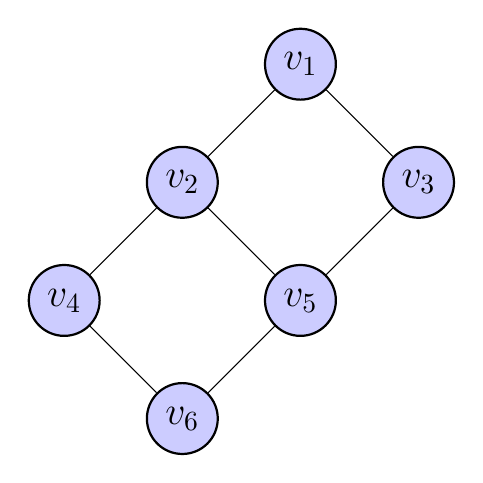
\begin{tikzpicture}[
  scale=1.5,
  vnode/.style={circle, fill=blue!20, draw=black, thick, minimum size=9mm, inner sep=0pt, font=\Large}
]
  % Vértices
  \node[vnode] (v1) at (2, 3) {$v_1$};
  \node[vnode] (v2) at (1, 2) {$v_2$};
  \node[vnode] (v3) at (3, 2) {$v_3$};
  \node[vnode] (v4) at (0, 1) {$v_4$};
  \node[vnode] (v5) at (2, 1) {$v_5$};
  \node[vnode] (v6) at (1, 0) {$v_6$};

  % Aristas
  \foreach \from/\to in {v1/v2, v1/v3, v2/v4, v2/v5, v3/v5, v4/v6, v5/v6}
    \draw (\from) -- (\to);
\end{tikzpicture}
}}}$
            &
            $\vcenter{\hbox{$\displaystyle \begin{pmatrix}
         0 & 1 & 1 & 0 & 0 & 0 \\
         1 & 0 & 0 & 1 & 1 & 0 \\
         1 & 0 & 0 & 0 & 1 & 0 \\
         0 & 1 & 0 & 0 & 0 & 1 \\
         0 & 1 & 1 & 0 & 0 & 1 \\
         0 & 0 & 0 & 1 & 1 & 0
      \end{pmatrix}$}}$ \\
            \noalign{\vspace{6pt}}
         \end{tabular}%
      } \\
      \hline
      \multicolumn{3}{c}{\textbf{Topología de adyacencia}} \\
      \hline
      Abiertos subbásicos & Vecindades mínimas & Topología \\
      \hline
         ${A_{v_1}=\{v_2,v_3\}}$\par
         ${A_{v_2}=\{v_1,v_4,v_5\}}$\par
         ${A_{v_3}=\{v_1,v_5\}}$\par
         ${A_{v_4}=\{v_2,v_6\}}$\par
         ${A_{v_5}=\{v_2,v_3,v_6\}}$\par
         ${A_{v_6}=\{v_4,v_5\}}$
      &
         ${U_{v_1}=\{v_1,v_5\}}$\par
         ${U_{v_2}=\{v_2\}}$\par
         ${U_{v_3}=\{v_2,v_3\}}$\par
         ${U_{v_4}=\{v_4,v_5\}}$\par
         ${U_{v_5}=\{v_5\}}$\par
         ${U_{v_6}=\{v_2,v_6\}}$
      &
         $\{\emptyset,$ $\{v_2\},$ $\{v_5\},$ $\{v_1,v_5\},$ $\{v_2,v_3\},$ $\{v_2,v_5\},$ $\{v_2,v_6\},$ $\{v_4,v_5\},$ $\{v_1,v_2,v_5\},$ $\{v_1,v_4,v_5\},$ $\{v_2,v_3,v_5\},$ $\{v_2,v_3,v_6\},$ $\{v_2,v_4,v_5\},$ $\{v_2,v_5,v_6\},$ $\{v_1,v_2,v_3,v_5\},$ $\{v_1,v_2,v_4,v_5\},$ $\{v_1,v_2,v_5,v_6\},$ $\{v_2,v_3,v_4,v_5\},$ $\{v_2,v_3,v_5,v_6\},$ $\{v_2,v_4,v_5,v_6\},$ $\{v_1,v_2,v_3,v_4,v_5\},$ $\{v_1,v_2,v_3,v_5,v_6\},$ $\{v_1,v_2,v_4,v_5,v_6\},$ $\{v_2,v_3,v_4,v_5,v_6\},$ $\{v_1,\allowbreak v_2,\allowbreak v_3,\allowbreak v_4,\allowbreak v_5,\allowbreak v_6\}\}$ \\[6pt]
      \hline
      \multicolumn{3}{c}{\textbf{Topología de incidencia}} \\
      \hline
      Abiertos subbásicos & Vecindades mínimas & Topología \\
      \hline
         ${e_{1}=\{v_1,v_2\}}$\par
         ${e_{2}=\{v_1,v_3\}}$\par
         ${e_{3}=\{v_2,v_4\}}$\par
         ${e_{4}=\{v_2,v_5\}}$\par
         ${e_{5}=\{v_3,v_5\}}$\par
         ${e_{6}=\{v_4,v_6\}}$\par
         ${e_{7}=\{v_5,v_6\}}$
      &
         ${U_{v_1}=\{v_1\}}$\par
         ${U_{v_2}=\{v_2\}}$\par
         ${U_{v_3}=\{v_3\}}$\par
         ${U_{v_4}=\{v_4\}}$\par
         ${U_{v_5}=\{v_5\}}$\par
         ${U_{v_6}=\{v_6\}}$
      &
         $\wp\left(V\left(G_3\right)\right)$ \\[6pt]
      \hline
   \end{tabular}
   \caption{Topologías de adyacencia e incidencia de $G_3$}
   \label{tab:topologias_G_3}

   \vspace{2em}
   \begin{minipage}{\textwidth}
      \normalsize
      El grafo $G_3$ es un ejemplo de retículo distributivo.
   \end{minipage}
\end{table}

\clearpage
\begin{table}[p]
   \centering
   \footnotesize
   \renewcommand{\arraystretch}{1.15}
   \begin{tabular}{@{}>{\centering\arraybackslash}m{0.3033\textwidth}>{\centering\arraybackslash}m{0.3033\textwidth}>{\centering\arraybackslash}m{0.3033\textwidth}@{}}
      \hline
      \multicolumn{3}{@{}c@{}}{%
         \begin{tabular}{@{}>{\centering\arraybackslash}m{\dimexpr0.455\textwidth+\tabcolsep\relax}>{\centering\arraybackslash}m{\dimexpr0.455\textwidth+\tabcolsep\relax}@{}}
            $M_5$ & Matriz de adyacencia \\
            \hline
            \noalign{\vspace{6pt}}
            \rule{0pt}{0pt}$\vcenter{\hbox{\resizebox{0.25\textwidth}{!}{% $M_5$, ejemplo de retículo que no es distributivo
%Incluido
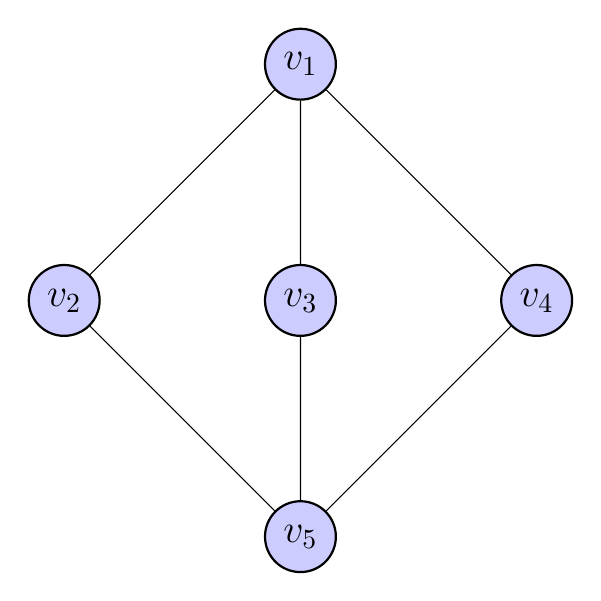
\begin{tikzpicture}[
  scale=1.5,
  vnode/.style={circle, fill=blue!20, draw=black, thick, minimum size=9mm, inner sep=0pt, font=\Large}
]
  % Vértices
  \node[vnode] (v1) at (2, 4) {$v_1$};
  \node[vnode] (v2) at (0, 2) {$v_2$};
  \node[vnode] (v3) at (2, 2) {$v_3$};
  \node[vnode] (v4) at (4, 2) {$v_4$};
  \node[vnode] (v5) at (2, 0) {$v_5$};

  % Aristas
  \foreach \from/\to in {v1/v2, v1/v3, v1/v4, v2/v5, v3/v5, v4/v5}
    \draw (\from) -- (\to);
\end{tikzpicture}
}}}$
            &
            $\vcenter{\hbox{$\displaystyle \begin{pmatrix}
         0 & 1 & 1 & 1 & 0 \\
         1 & 0 & 0 & 0 & 1 \\
         1 & 0 & 0 & 0 & 1 \\
         1 & 0 & 0 & 0 & 1 \\
         0 & 1 & 1 & 1 & 0
      \end{pmatrix}$}}$ \\
            \noalign{\vspace{6pt}}
         \end{tabular}%
      } \\
      \hline
      \multicolumn{3}{c}{\textbf{Topología de adyacencia}} \\
      \hline
      Abiertos subbásicos & Vecindades mínimas & Topología \\
      \hline
         ${A_{v_1}=\{v_2,v_3,v_4\}}$\par
         ${A_{v_2}=\{v_1,v_5\}}$\par
         ${A_{v_3}=\{v_1,v_5\}}$\par
         ${A_{v_4}=\{v_1,v_5\}}$\par
         ${A_{v_5}=\{v_2,v_3,v_4\}}$
      &
         ${U_{v_1}=\{v_1,v_5\}}$\par
         ${U_{v_2}=\{v_2,v_3,v_4\}}$\par
         ${U_{v_3}=\{v_2,v_3,v_4\}}$\par
         ${U_{v_4}=\{v_2,v_3,v_4\}}$\par
         ${U_{v_5}=\{v_1,v_5\}}$
      &
         $\{\emptyset,$ $\{v_1,v_5\},$ $\{v_2,v_3,v_4\},$ $\{v_1,v_2,v_3,v_4,v_5\}\}$ \\[6pt]
      \hline
      \multicolumn{3}{c}{\textbf{Topología de incidencia}} \\
      \hline
      Abiertos subbásicos & Vecindades mínimas & Topología \\
      \hline
         ${e_{1}=\{v_1,v_2\}}$\par
         ${e_{2}=\{v_1,v_3\}}$\par
         ${e_{3}=\{v_1,v_4\}}$\par
         ${e_{4}=\{v_2,v_5\}}$\par
         ${e_{5}=\{v_3,v_5\}}$\par
         ${e_{6}=\{v_4,v_5\}}$
      &
         ${U_{v_1}=\{v_1\}}$\par
         ${U_{v_2}=\{v_2\}}$\par
         ${U_{v_3}=\{v_3\}}$\par
         ${U_{v_4}=\{v_4\}}$\par
         ${U_{v_5}=\{v_5\}}$
      &
         $\wp\left(V\left(M_5\right)\right)$ \\[6pt]
      \hline
   \end{tabular}
   \caption{Topologías de adyacencia e incidencia de $M_5$}
   \label{tab:topologias_M_5}

   \vspace{2em}
   \begin{minipage}{\textwidth}
      \normalsize
      El grafo $M_5$ es un ejemplo de retículo que no es distributivo.
   \end{minipage}
\end{table}

\clearpage
\begin{table}[p]
   \centering
   \footnotesize
   \renewcommand{\arraystretch}{1.15}
   \begin{tabular}{@{}>{\centering\arraybackslash}m{0.3033\textwidth}>{\centering\arraybackslash}m{0.3033\textwidth}>{\centering\arraybackslash}m{0.3033\textwidth}@{}}
      \hline
      \multicolumn{3}{@{}c@{}}{%
         \begin{tabular}{@{}>{\centering\arraybackslash}m{\dimexpr0.455\textwidth+\tabcolsep\relax}>{\centering\arraybackslash}m{\dimexpr0.455\textwidth+\tabcolsep\relax}@{}}
            $N_5$ & Matriz de adyacencia \\
            \hline
            \noalign{\vspace{6pt}}
            \rule{0pt}{0pt}$\vcenter{\hbox{\resizebox{0.25\textwidth}{!}{% $N_5$, ejemplo de retículo que no es distributivo
% Incluido
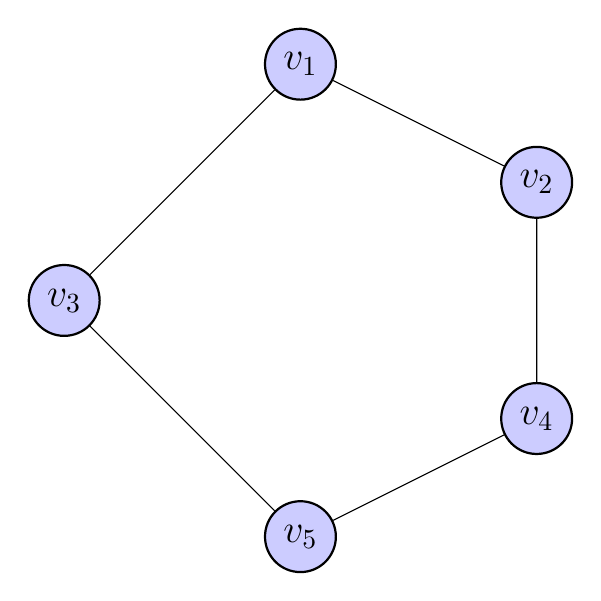
\begin{tikzpicture}[
  scale=1.5,
  vnode/.style={circle, fill=blue!20, draw=black, thick, minimum size=9mm, inner sep=0pt, font=\Large}
]
  % Vértices
  \node[vnode] (v1) at (2, 4) {$v_1$};
  \node[vnode] (v2) at (4, 3) {$v_2$};
  \node[vnode] (v3) at (0, 2) {$v_3$};
  \node[vnode] (v4) at (4, 1) {$v_4$};
  \node[vnode] (v5) at (2, 0) {$v_5$};

  % Aristas
  \foreach \from/\to in {v1/v2, v1/v3, v2/v4, v3/v5, v4/v5}
    \draw (\from) -- (\to);
\end{tikzpicture}
}}}$
            &
            $\vcenter{\hbox{$\displaystyle \begin{pmatrix}
         0 & 1 & 1 & 0 & 0 \\
         1 & 0 & 0 & 1 & 0 \\
         1 & 0 & 0 & 0 & 1 \\
         0 & 1 & 0 & 0 & 1 \\
         0 & 0 & 1 & 1 & 0
      \end{pmatrix}$}}$ \\
            \noalign{\vspace{6pt}}
         \end{tabular}%
      } \\
      \hline
      \multicolumn{3}{c}{\textbf{Topología de adyacencia}} \\
      \hline
      Abiertos subbásicos & Vecindades mínimas & Topología \\
      \hline
         ${A_{v_1}=\{v_2,v_3\}}$\par
         ${A_{v_2}=\{v_1,v_4\}}$\par
         ${A_{v_3}=\{v_1,v_5\}}$\par
         ${A_{v_4}=\{v_2,v_5\}}$\par
         ${A_{v_5}=\{v_3,v_4\}}$
      &
         ${U_{v_1}=\{v_1\}}$\par
         ${U_{v_2}=\{v_2\}}$\par
         ${U_{v_3}=\{v_3\}}$\par
         ${U_{v_4}=\{v_4\}}$\par
         ${U_{v_5}=\{v_5\}}$
      &
         $\wp\left(V\left(N_5\right)\right)$ \\[6pt]
      \hline
      \multicolumn{3}{c}{\textbf{Topología de incidencia}} \\
      \hline
      Abiertos subbásicos & Vecindades mínimas & Topología \\
      \hline
         ${e_{1}=\{v_1,v_2\}}$\par
         ${e_{2}=\{v_1,v_3\}}$\par
         ${e_{3}=\{v_2,v_4\}}$\par
         ${e_{4}=\{v_3,v_5\}}$\par
         ${e_{5}=\{v_4,v_5\}}$
      &
         ${U_{v_1}=\{v_1\}}$\par
         ${U_{v_2}=\{v_2\}}$\par
         ${U_{v_3}=\{v_3\}}$\par
         ${U_{v_4}=\{v_4\}}$\par
         ${U_{v_5}=\{v_5\}}$
      &
         $\wp\left(V\left(N_5\right)\right)$ \\[6pt]
      \hline
   \end{tabular}
   \caption{Topologías de adyacencia e incidencia de $N_5$}
   \label{tab:topologias_N_5}

   \vspace{2em}
   \begin{minipage}{\textwidth}
      \normalsize
      El grafo $N_5$ es un ejemplo de retículo que no es distributivo.
   \end{minipage}
\end{table}

\clearpage
\begin{table}[p]
   \centering
   \footnotesize
   \renewcommand{\arraystretch}{1.15}
   \begin{tabular}{@{}>{\centering\arraybackslash}m{0.3033\textwidth}>{\centering\arraybackslash}m{0.3033\textwidth}>{\centering\arraybackslash}m{0.3033\textwidth}@{}}
      \hline
      \multicolumn{3}{@{}c@{}}{%
         \begin{tabular}{@{}>{\centering\arraybackslash}m{\dimexpr0.455\textwidth+\tabcolsep\relax}>{\centering\arraybackslash}m{\dimexpr0.455\textwidth+\tabcolsep\relax}@{}}
            $G_4$ & Matriz de adyacencia \\
            \hline
            \noalign{\vspace{6pt}}
            \rule{0pt}{0pt}$\vcenter{\hbox{\resizebox{0.17\textwidth}{!}{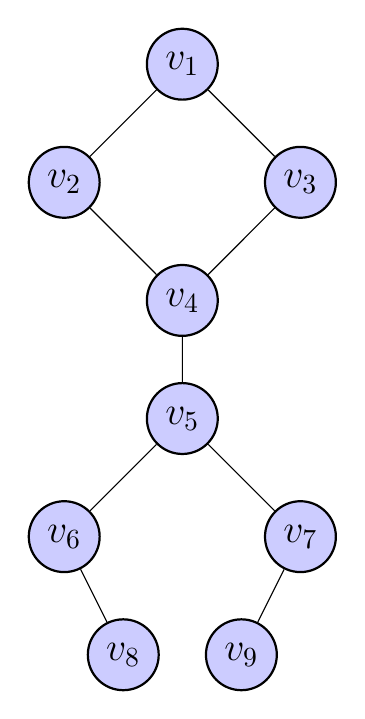
\begin{tikzpicture}[
  scale=1.5,
  vnode/.style={circle, fill=blue!20, draw=black, thick, minimum size=9mm, inner sep=0pt, font=\Large}
]
  % Vértices
  \node[vnode] (v1) at (1, 5) {$v_1$};
  \node[vnode] (v2) at (0, 4) {$v_2$};
  \node[vnode] (v3) at (2, 4) {$v_3$};
  \node[vnode] (v4) at (1, 3) {$v_4$};
  \node[vnode] (v5) at (1, 2) {$v_5$};
  \node[vnode] (v6) at (0, 1) {$v_6$};
  \node[vnode] (v7) at (2, 1) {$v_7$};
  \node[vnode] (v8) at (0.5, 0) {$v_8$};
  \node[vnode] (v9) at (1.5, 0) {$v_9$};

  % Aristas
  \foreach \from/\to in {v1/v2, v1/v3, v2/v4, v3/v4, v4/v5,
                         v5/v6, v5/v7, v6/v8, v7/v9}
    \draw (\from) -- (\to);
\end{tikzpicture}
}}}$
            &
            $\vcenter{\hbox{$\displaystyle \begin{pmatrix}
         0 & 1 & 1 & 0 & 0 & 0 & 0 & 0 & 0 \\
         1 & 0 & 0 & 1 & 0 & 0 & 0 & 0 & 0 \\
         1 & 0 & 0 & 1 & 0 & 0 & 0 & 0 & 0 \\
         0 & 1 & 1 & 0 & 1 & 0 & 0 & 0 & 0 \\
         0 & 0 & 0 & 1 & 0 & 1 & 1 & 0 & 0 \\
         0 & 0 & 0 & 0 & 1 & 0 & 0 & 1 & 0 \\
         0 & 0 & 0 & 0 & 1 & 0 & 0 & 0 & 1 \\
         0 & 0 & 0 & 0 & 0 & 1 & 0 & 0 & 0 \\
         0 & 0 & 0 & 0 & 0 & 0 & 1 & 0 & 0
      \end{pmatrix}$}}$ \\
            \noalign{\vspace{6pt}}
         \end{tabular}%
      } \\
      \hline
      \multicolumn{3}{c}{\textbf{Topología de adyacencia}} \\
      \hline
      Abiertos subbásicos & Vecindades mínimas & Topología \\
      \hline
         ${A_{v_1}=\{v_2,v_3\}}$\par
         ${A_{v_2}=\{v_1,v_4\}}$\par
         ${A_{v_3}=\{v_1,v_4\}}$\par
         ${A_{v_4}=\{v_2,v_3,v_5\}}$\par
         ${A_{v_5}=\{v_4,v_6,v_7\}}$\par
         ${A_{v_6}=\{v_5,v_8\}}$\par
         ${A_{v_7}=\{v_5,v_9\}}$\par
         ${A_{v_8}=\{v_6\}}$\par
         ${A_{v_9}=\{v_7\}}$
      &
         ${U_{v_1}=\{v_1,v_4\}}$\par
         ${U_{v_2}=\{v_2,v_3\}}$\par
         ${U_{v_3}=\{v_2,v_3\}}$\par
         ${U_{v_4}=\{v_4\}}$\par
         ${U_{v_5}=\{v_5\}}$\par
         ${U_{v_6}=\{v_6\}}$\par
         ${U_{v_7}=\{v_7\}}$\par
         ${U_{v_8}=\{v_5,v_8\}}$\par
         ${U_{v_9}=\{v_5,v_9\}}$
      &
                  No discreta, con 120 abiertos \\[6pt]
      \hline
      \multicolumn{3}{c}{\textbf{Topología de incidencia}} \\
      \hline
      Abiertos subbásicos & Vecindades mínimas & Topología \\
      \hline
         ${e_{1}=\{v_1,v_2\}}$\par
         ${e_{2}=\{v_1,v_3\}}$\par
         ${e_{3}=\{v_2,v_4\}}$\par
         ${e_{4}=\{v_3,v_4\}}$\par
         ${e_{5}=\{v_4,v_5\}}$\par
         ${e_{6}=\{v_5,v_6\}}$\par
         ${e_{7}=\{v_5,v_7\}}$\par
         ${e_{8}=\{v_6,v_8\}}$\par
         ${e_{9}=\{v_7,v_9\}}$
      &
         ${U_{v_1}=\{v_1\}}$\par
         ${U_{v_2}=\{v_2\}}$\par
         ${U_{v_3}=\{v_3\}}$\par
         ${U_{v_4}=\{v_4\}}$\par
         ${U_{v_5}=\{v_5\}}$\par
         ${U_{v_6}=\{v_6\}}$\par
         ${U_{v_7}=\{v_7\}}$\par
         ${U_{v_8}=\{v_6,v_8\}}$\par
         ${U_{v_9}=\{v_7,v_9\}}$
      &
                  No discreta, con 288 abiertos \\[6pt]      \hline
   \end{tabular}
   \caption{Topologías de adyacencia e incidencia de $G_4$}
   \label{tab:topologias_G_4}
\end{table}

\clearpage
\begin{table}[p]
   \centering
   \footnotesize
   \renewcommand{\arraystretch}{1.15}
   \begin{tabular}{@{}>{\centering\arraybackslash}m{0.3033\textwidth}>{\centering\arraybackslash}m{0.3033\textwidth}>{\centering\arraybackslash}m{0.3033\textwidth}@{}}
      \hline
      \multicolumn{3}{@{}c@{}}{%
         \begin{tabular}{@{}>{\centering\arraybackslash}m{\dimexpr0.455\textwidth+\tabcolsep\relax}>{\centering\arraybackslash}m{\dimexpr0.455\textwidth+\tabcolsep\relax}@{}}
            $G_5$ & Matriz de adyacencia \\
            \hline
            \noalign{\vspace{6pt}}
            \rule{0pt}{0pt}$\vcenter{\hbox{\resizebox{0.25\textwidth}{!}{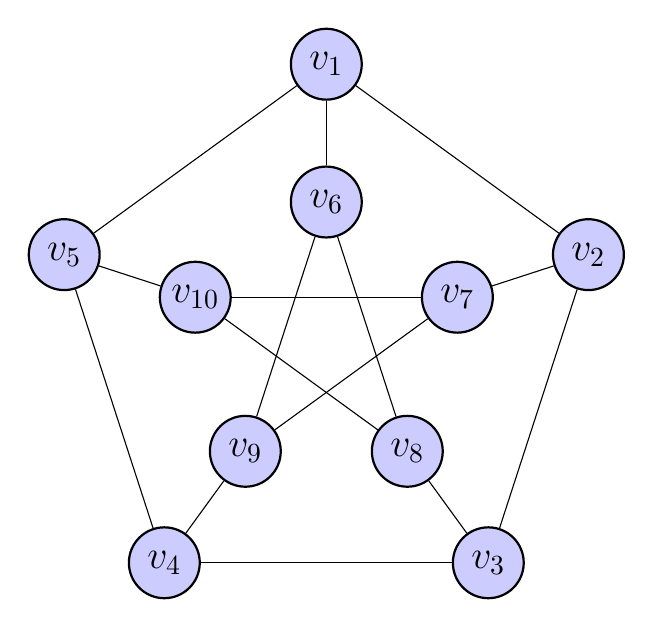
\begin{tikzpicture}[
  scale=1,
  vnode/.style={circle, fill=blue!20, draw=black, thick, minimum size=9mm, inner sep=0pt, font=\Large}
]
  % Vértices del pentágono exterior (en sentido horario desde arriba)
  \node[vnode] (v1) at (90:3.5)  {$v_1$};
  \node[vnode] (v2) at (18:3.5)  {$v_2$};
  \node[vnode] (v3) at (-54:3.5) {$v_3$};
  \node[vnode] (v4) at (-126:3.5) {$v_4$};
  \node[vnode] (v5) at (162:3.5) {$v_5$};

  % Vértices de la estrella interior (en sentido horario desde arriba)
  \node[vnode] (v6)  at (90:1.75)  {$v_6$};
  \node[vnode] (v7)  at (18:1.75)  {$v_7$};
  \node[vnode] (v8)  at (-54:1.75) {$v_8$};
  \node[vnode] (v9)  at (-126:1.75) {$v_9$};
  \node[vnode] (v10) at (162:1.75) {$v_{10}$};

  % Aristas
  \foreach \from/\to in {v1/v2, v2/v3, v3/v4, v4/v5, v5/v1,
                         v1/v6, v2/v7, v3/v8, v4/v9, v5/v10,
                         v6/v8, v8/v10, v10/v7, v7/v9, v9/v6}
    \draw (\from) -- (\to);
\end{tikzpicture}
}}}$
            &
            $\vcenter{\hbox{\tiny$\begin{pmatrix}
         0 & 1 & 0 & 0 & 1 & 1 & 0 & 0 & 0 & 0 \\
         1 & 0 & 1 & 0 & 0 & 0 & 1 & 0 & 0 & 0 \\
         0 & 1 & 0 & 1 & 0 & 0 & 0 & 1 & 0 & 0 \\
         0 & 0 & 1 & 0 & 1 & 0 & 0 & 0 & 1 & 0 \\
         1 & 0 & 0 & 1 & 0 & 0 & 0 & 0 & 0 & 1 \\
         1 & 0 & 0 & 0 & 0 & 0 & 0 & 1 & 1 & 0 \\
         0 & 1 & 0 & 0 & 0 & 0 & 0 & 0 & 1 & 1 \\
         0 & 0 & 1 & 0 & 0 & 1 & 0 & 0 & 0 & 1 \\
         0 & 0 & 0 & 1 & 0 & 1 & 1 & 0 & 0 & 0 \\
         0 & 0 & 0 & 0 & 1 & 0 & 1 & 1 & 0 & 0
      \end{pmatrix}$}}$ \\
            \noalign{\vspace{6pt}}
         \end{tabular}%
      } \\
      \hline
      \multicolumn{3}{c}{\textbf{Topología de adyacencia}} \\
      \hline
      Abiertos subbásicos & Vecindades mínimas & Topología \\
      \hline
         ${A_{v_1}=\{v_2,v_5,v_6\}}$\par
         ${A_{v_2}=\{v_1,v_3,v_7\}}$\par
         ${A_{v_3}=\{v_2,v_4,v_8\}}$\par
         ${A_{v_4}=\{v_3,v_5,v_9\}}$\par
         ${A_{v_5}=\{v_1,v_4,v_{10}\}}$\par
         ${A_{v_6}=\{v_1,v_8,v_9\}}$\par
         ${A_{v_7}=\{v_2,v_9,v_{10}\}}$\par
         ${A_{v_8}=\{v_3,v_6,v_{10}\}}$\par
         ${A_{v_9}=\{v_4,v_6,v_7\}}$\par
         ${A_{v_{10}}=\{v_5,v_7,v_8\}}$
      &
         ${U_{v_1}=\{v_1\}}$\par
         ${U_{v_2}=\{v_2\}}$\par
         ${U_{v_3}=\{v_3\}}$\par
         ${U_{v_4}=\{v_4\}}$\par
         ${U_{v_5}=\{v_5\}}$\par
         ${U_{v_6}=\{v_6\}}$\par
         ${U_{v_7}=\{v_7\}}$\par
         ${U_{v_8}=\{v_8\}}$\par
         ${U_{v_9}=\{v_9\}}$\par
         ${U_{v_{10}}=\{v_{10}\}}$
      &
         $\wp\left(V\left(G_5\right)\right)$ \\[6pt]
      \hline
      \multicolumn{3}{c}{\textbf{Topología de incidencia}} \\
      \hline
      Abiertos subbásicos & Vecindades mínimas & Topología \\
      \hline
         ${e_{1}=\{v_1,v_2\}}$\par
         ${e_{2}=\{v_1,v_5\}}$\par
         ${e_{3}=\{v_1,v_6\}}$\par
         ${e_{4}=\{v_2,v_3\}}$\par
         ${e_{5}=\{v_2,v_7\}}$\par
         ${e_{6}=\{v_3,v_4\}}$\par
         ${e_{7}=\{v_3,v_8\}}$\par
         ${e_{8}=\{v_4,v_5\}}$\par
         ${e_{9}=\{v_4,v_9\}}$\par
         ${e_{10}=\{v_5,v_{10}\}}$\par
         ${e_{11}=\{v_6,v_8\}}$\par
         ${e_{12}=\{v_6,v_9\}}$\par
         ${e_{13}=\{v_7,v_9\}}$\par
         ${e_{14}=\{v_7,v_{10}\}}$\par
         ${e_{15}=\{v_8,v_{10}\}}$
      &
         ${U_{v_1}=\{v_1\}}$\par
         ${U_{v_2}=\{v_2\}}$\par
         ${U_{v_3}=\{v_3\}}$\par
         ${U_{v_4}=\{v_4\}}$\par
         ${U_{v_5}=\{v_5\}}$\par
         ${U_{v_6}=\{v_6\}}$\par
         ${U_{v_7}=\{v_7\}}$\par
         ${U_{v_8}=\{v_8\}}$\par
         ${U_{v_9}=\{v_9\}}$\par
         ${U_{v_{10}}=\{v_{10}\}}$
      &
         $\wp\left(V\left(G_5\right)\right)$ \\[6pt]
      \hline
   \end{tabular}
   \caption{Topologías de adyacencia e incidencia de $G_5$}
   \label{tab:topologias_G_5}

   \vspace{1em}
   \begin{minipage}{\textwidth}
      \normalsize
      El grafo $G_5$ es conocido como \textit{Grafo de Petersen}.
   \end{minipage}
\end{table}

\clearpage
\begin{table}[p]
   \centering
   \footnotesize
   \renewcommand{\arraystretch}{1.15}
   \begin{tabular}{@{}>{\centering\arraybackslash}m{0.3033\textwidth}>{\centering\arraybackslash}m{0.3033\textwidth}>{\centering\arraybackslash}m{0.3033\textwidth}@{}}
      \hline
      \multicolumn{3}{@{}c@{}}{%
         \begin{tabular}{@{}>{\centering\arraybackslash}m{\dimexpr0.455\textwidth+\tabcolsep\relax}>{\centering\arraybackslash}m{\dimexpr0.455\textwidth+\tabcolsep\relax}@{}}
            $G_6$ & Matriz de adyacencia \\
            \hline
            \noalign{\vspace{6pt}}
            \rule{0pt}{0pt}$\vcenter{\hbox{\resizebox{0.25\textwidth}{!}{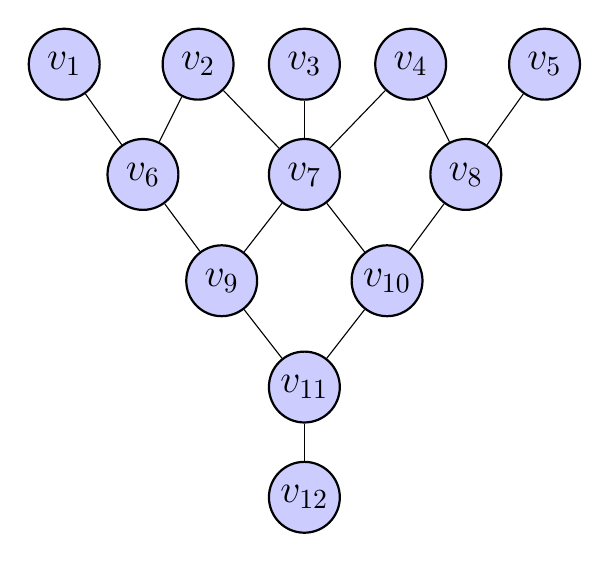
\begin{tikzpicture}[
  scale=1,
  vnode/.style={circle, fill=blue!20, draw=black, thick, minimum size=9mm, inner sep=0pt, font=\Large}
]
  % Vértices
  \node[vnode] (v1)  at (0.4, 5.5) {$v_1$};
  \node[vnode] (v2)  at (2.1, 5.5) {$v_2$};
  \node[vnode] (v3)  at (3.45, 5.5) {$v_3$};
  \node[vnode] (v4)  at (4.8, 5.5) {$v_4$};
  \node[vnode] (v5)  at (6.5, 5.5) {$v_5$};
  \node[vnode] (v6)  at (1.4, 4.1) {$v_6$};
  \node[vnode] (v7)  at (3.45, 4.1) {$v_7$};
  \node[vnode] (v8)  at (5.5, 4.1) {$v_8$};
  \node[vnode] (v9)  at (2.4, 2.75) {$v_9$};
  \node[vnode] (v10) at (4.5, 2.75) {$v_{10}$};
  \node[vnode] (v11) at (3.45, 1.4) {$v_{11}$};
  \node[vnode] (v12) at (3.45, 0) {$v_{12}$};

  % Aristas
  \foreach \from/\to in {v1/v6, v2/v6, v2/v7, v3/v7, v4/v7, v4/v8, v5/v8,
                         v6/v9, v7/v9, v7/v10, v8/v10, v9/v11, v10/v11, v11/v12}
    \draw (\from) -- (\to);
\end{tikzpicture}
}}}$
            &
            $\vcenter{\hbox{\tiny$\setcounter{MaxMatrixCols}{12}\begin{pmatrix}
         0 & 0 & 0 & 0 & 0 & 1 & 0 & 0 & 0 & 0 & 0 & 0 \\
         0 & 0 & 0 & 0 & 0 & 1 & 1 & 0 & 0 & 0 & 0 & 0 \\
         0 & 0 & 0 & 0 & 0 & 0 & 1 & 0 & 0 & 0 & 0 & 0 \\
         0 & 0 & 0 & 0 & 0 & 0 & 1 & 1 & 0 & 0 & 0 & 0 \\
         0 & 0 & 0 & 0 & 0 & 0 & 0 & 1 & 0 & 0 & 0 & 0 \\
         1 & 1 & 0 & 0 & 0 & 0 & 0 & 0 & 1 & 0 & 0 & 0 \\
         0 & 1 & 1 & 1 & 0 & 0 & 0 & 0 & 1 & 1 & 0 & 0 \\
         0 & 0 & 0 & 1 & 1 & 0 & 0 & 0 & 0 & 1 & 0 & 0 \\
         0 & 0 & 0 & 0 & 0 & 1 & 1 & 0 & 0 & 0 & 1 & 0 \\
         0 & 0 & 0 & 0 & 0 & 0 & 1 & 1 & 0 & 0 & 1 & 0 \\
         0 & 0 & 0 & 0 & 0 & 0 & 0 & 0 & 1 & 1 & 0 & 1 \\
         0 & 0 & 0 & 0 & 0 & 0 & 0 & 0 & 0 & 0 & 1 & 0
      \end{pmatrix}$}}$ \\
            \noalign{\vspace{6pt}}
         \end{tabular}%
      } \\
      \hline
      \multicolumn{3}{c}{\textbf{Topología de adyacencia}} \\
      \hline
      Abiertos subbásicos & Vecindades mínimas & Topología \\
      \hline
         ${A_{v_1}=\{v_6\}}$\par
         ${A_{v_2}=\{v_6,v_7\}}$\par
         ${A_{v_3}=\{v_7\}}$\par
         ${A_{v_4}=\{v_7,v_8\}}$\par
         ${A_{v_5}=\{v_8\}}$\par
         ${A_{v_6}=\{v_1,v_2,v_9\}}$\par
         ${A_{v_7}=\{v_2,v_3,v_4,v_9,v_{10}\}}$\par
         ${A_{v_8}=\{v_4,v_5,v_{10}\}}$\par
         ${A_{v_9}=\{v_6,v_7,v_{11}\}}$\par
         ${A_{v_{10}}=\{v_7,v_8,v_{11}\}}$\par
         ${A_{v_{11}}=\{v_9,v_{10},v_{12}\}}$\par
         ${A_{v_{12}}=\{v_{11}\}}$
      &
         ${U_{v_1}=\{v_1,v_2,v_9\}}$\par
         ${U_{v_2}=\{v_2,v_9\}}$\par
         ${U_{v_3}=\{v_2,v_3,v_4,v_9,v_{10}\}}$\par
         ${U_{v_4}=\{v_4,v_{10}\}}$\par
         ${U_{v_5}=\{v_4,v_5,v_{10}\}}$\par
         ${U_{v_6}=\{v_6\}}$\par
         ${U_{v_7}=\{v_7\}}$\par
         ${U_{v_8}=\{v_8\}}$\par
         ${U_{v_9}=\{v_9\}}$\par
         ${U_{v_{10}}=\{v_{10}\}}$\par
         ${U_{v_{11}}=\{v_{11}\}}$\par
         ${U_{v_{12}}=\{v_9,v_{10},v_{12}\}}$
      &
         No discreta, con 528 abiertos \\[6pt]
      \hline
      \multicolumn{3}{c}{\textbf{Topología de incidencia}} \\
      \hline
      Abiertos subbásicos & Vecindades mínimas & Topología \\
      \hline
         ${e_{1}=\{v_1,v_6\}}$\par
         ${e_{2}=\{v_2,v_6\}}$\par
         ${e_{3}=\{v_2,v_7\}}$\par
         ${e_{4}=\{v_3,v_7\}}$\par
         ${e_{5}=\{v_4,v_7\}}$\par
         ${e_{6}=\{v_4,v_8\}}$\par
         ${e_{7}=\{v_5,v_8\}}$\par
         ${e_{8}=\{v_6,v_9\}}$\par
         ${e_{9}=\{v_7,v_9\}}$\par
         ${e_{10}=\{v_7,v_{10}\}}$\par
         ${e_{11}=\{v_8,v_{10}\}}$\par
         ${e_{12}=\{v_9,v_{11}\}}$\par
         ${e_{13}=\{v_{10},v_{11}\}}$\par
         ${e_{14}=\{v_{11},v_{12}\}}$
      &
         ${U_{v_1}=\{v_1,v_6\}}$\par
         ${U_{v_2}=\{v_2\}}$\par
         ${U_{v_3}=\{v_3,v_7\}}$\par
         ${U_{v_4}=\{v_4\}}$\par
         ${U_{v_5}=\{v_5,v_8\}}$\par
         ${U_{v_6}=\{v_6\}}$\par
         ${U_{v_7}=\{v_7\}}$\par
         ${U_{v_8}=\{v_8\}}$\par
         ${U_{v_9}=\{v_9\}}$\par
         ${U_{v_{10}}=\{v_{10}\}}$\par
         ${U_{v_{11}}=\{v_{11}\}}$\par
         ${U_{v_{12}}=\{v_{11},v_{12}\}}$
      &
         No discreta, con 1296 abiertos \\[6pt]
      \hline
   \end{tabular}
   \caption{Topologías de adyacencia e incidencia de $G_6$}
   \label{tab:topologias_G_6}

   \vspace{1em}
   \begin{minipage}{\textwidth}
      \normalsize
      El grafo $G_6$ es un fragmento del \textit{Grafo de Young-Fibonacci}.
   \end{minipage}
\end{table}

\clearpage
\begin{table}[p]
   \centering
   \footnotesize
   \renewcommand{\arraystretch}{1.15}
   \begin{tabular}{@{}>{\centering\arraybackslash}m{0.3033\textwidth}>{\centering\arraybackslash}m{0.3033\textwidth}>{\centering\arraybackslash}m{0.3033\textwidth}@{}}
      \hline
      \multicolumn{3}{@{}c@{}}{%
         \begin{tabular}{@{}>{\centering\arraybackslash}m{\dimexpr0.455\textwidth+\tabcolsep\relax}>{\centering\arraybackslash}m{\dimexpr0.455\textwidth+\tabcolsep\relax}@{}}
            $T_1$ & Matriz de adyacencia \\
            \hline
            \noalign{\vspace{6pt}}
            \rule{0pt}{0pt}$\vcenter{\hbox{\resizebox{0.25\textwidth}{!}{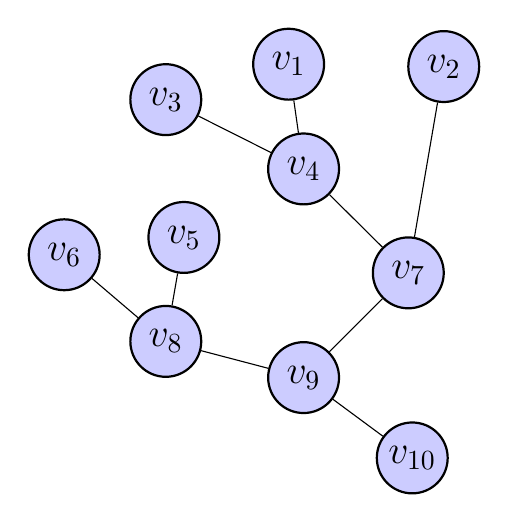
\begin{tikzpicture}[
  scale=1,
  vnode/.style={circle, fill=blue!20, draw=black, thick, minimum size=9mm, inner sep=0pt, font=\Large}
]
  % Vértices
  \node[vnode] (v1) at (3.73, 5.25) {$v_1$};
  \node[vnode] (v2) at (5.70, 5.22) {$v_2$};
  \node[vnode] (v3) at (2.17, 4.80) {$v_3$};
  \node[vnode] (v4) at (3.92, 3.92) {$v_4$};
  \node[vnode] (v5) at (2.40, 3.05) {$v_5$};
  \node[vnode] (v6) at (0.88, 2.83) {$v_6$};
  \node[vnode] (v7) at (5.25, 2.60) {$v_7$};
  \node[vnode] (v8) at (2.17, 1.73) {$v_8$};
  \node[vnode] (v9) at (3.92, 1.27) {$v_9$};
  \node[vnode] (v10) at (5.30, 0.25) {$v_{10}$};

  % Aristas
  \foreach \from/\to in {v1/v4, v2/v7, v3/v4, v4/v7, v5/v8, v6/v8, v7/v9, v8/v9, v9/v10}
    \draw (\from) -- (\to);
\end{tikzpicture}
}}}$
            &
            $\vcenter{\hbox{\scriptsize$\begin{pmatrix}
         0 & 0 & 0 & 1 & 0 & 0 & 0 & 0 & 0 & 0 \\
         0 & 0 & 0 & 0 & 0 & 0 & 1 & 0 & 0 & 0 \\
         0 & 0 & 0 & 1 & 0 & 0 & 0 & 0 & 0 & 0 \\
         1 & 0 & 1 & 0 & 0 & 0 & 1 & 0 & 0 & 0 \\
         0 & 0 & 0 & 0 & 0 & 0 & 0 & 1 & 0 & 0 \\
         0 & 0 & 0 & 0 & 0 & 0 & 0 & 1 & 0 & 0 \\
         0 & 1 & 0 & 1 & 0 & 0 & 0 & 0 & 1 & 0 \\
         0 & 0 & 0 & 0 & 1 & 1 & 0 & 0 & 1 & 0 \\
         0 & 0 & 0 & 0 & 0 & 0 & 1 & 1 & 0 & 1 \\
         0 & 0 & 0 & 0 & 0 & 0 & 0 & 0 & 1 & 0
      \end{pmatrix}$}}$ \\
            \noalign{\vspace{6pt}}
         \end{tabular}%
      } \\
      \hline
      \multicolumn{3}{c}{\textbf{Topología de adyacencia}} \\
      \hline
      Abiertos subbásicos & Vecindades mínimas & Topología \\
      \hline
         ${A_{v_1}=\{v_4\}}$\par
         ${A_{v_2}=\{v_7\}}$\par
         ${A_{v_3}=\{v_4\}}$\par
         ${A_{v_4}=\{v_1,v_3,v_7\}}$\par
         ${A_{v_5}=\{v_8\}}$\par
         ${A_{v_6}=\{v_8\}}$\par
         ${A_{v_7}=\{v_2,v_4,v_9\}}$\par
         ${A_{v_8}=\{v_5,v_6,v_9\}}$\par
         ${A_{v_9}=\{v_7,v_8,v_{10}\}}$\par
         ${A_{v_{10}}=\{v_9\}}$
      &
         ${U_{v_1}=\{v_1,v_3,v_7\}}$\par
         ${U_{v_2}=\{v_2,v_4,v_9\}}$\par
         ${U_{v_3}=\{v_1,v_3,v_7\}}$\par
         ${U_{v_4}=\{v_4\}}$\par
         ${U_{v_5}=\{v_5,v_6,v_9\}}$\par
         ${U_{v_6}=\{v_5,v_6,v_9\}}$\par
         ${U_{v_7}=\{v_7\}}$\par
         ${U_{v_8}=\{v_8\}}$\par
         ${U_{v_9}=\{v_9\}}$\par
         ${U_{v_{10}}=\{v_7,v_8,v_{10}\}}$
      &
         No discreta, con 64 abiertos \\[6pt]
      \hline
      \multicolumn{3}{c}{\textbf{Topología de incidencia}} \\
      \hline
      Abiertos subbásicos & Vecindades mínimas & Topología \\
      \hline
         ${e_{1}=\{v_1,v_4\}}$\par
         ${e_{2}=\{v_2,v_7\}}$\par
         ${e_{3}=\{v_3,v_4\}}$\par
         ${e_{4}=\{v_4,v_7\}}$\par
         ${e_{5}=\{v_5,v_8\}}$\par
         ${e_{6}=\{v_6,v_8\}}$\par
         ${e_{7}=\{v_7,v_9\}}$\par
         ${e_{8}=\{v_8,v_9\}}$\par
         ${e_{9}=\{v_9,v_{10}\}}$
      &
         ${U_{v_1}=\{v_1,v_4\}}$\par
         ${U_{v_2}=\{v_2,v_7\}}$\par
         ${U_{v_3}=\{v_3,v_4\}}$\par
         ${U_{v_4}=\{v_4\}}$\par
         ${U_{v_5}=\{v_5,v_8\}}$\par
         ${U_{v_6}=\{v_6,v_8\}}$\par
         ${U_{v_7}=\{v_7\}}$\par
         ${U_{v_8}=\{v_8\}}$\par
         ${U_{v_9}=\{v_9\}}$\par
         ${U_{v_{10}}=\{v_9,v_{10}\}}$
      &
         No discreta, con 225 abiertos \\[6pt]
      \hline
   \end{tabular}
   \caption{Topologías de adyacencia e incidencia de $T_1$}
   \label{tab:topologias_T_1}

   \vspace{2em}
   \begin{minipage}{\textwidth}
      \normalsize
      El grafo $T_1$ es un árbol.
   \end{minipage}
\end{table}

\clearpage
\begin{table}[p]
   \centering
   \footnotesize
   \renewcommand{\arraystretch}{1.15}
   \begin{tabular}{@{}>{\centering\arraybackslash}m{0.3033\textwidth}>{\centering\arraybackslash}m{0.3033\textwidth}>{\centering\arraybackslash}m{0.3033\textwidth}@{}}
      \hline
      \multicolumn{3}{@{}c@{}}{%
         \begin{tabular}{@{}>{\centering\arraybackslash}m{\dimexpr0.455\textwidth+\tabcolsep\relax}>{\centering\arraybackslash}m{\dimexpr0.455\textwidth+\tabcolsep\relax}@{}}
            $G_7$ & Matriz de adyacencia \\
            \hline
            \noalign{\vspace{6pt}}
            \rule{0pt}{0pt}$\vcenter{\hbox{\resizebox{0.45\textwidth}{!}{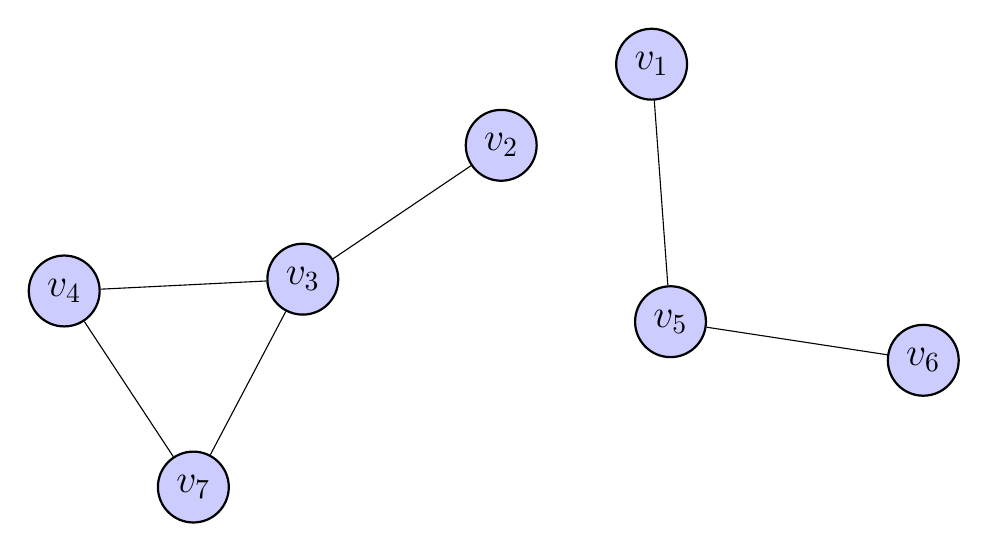
\begin{tikzpicture}[
  scale=1,
  vnode/.style={circle, fill=blue!20, draw=black, thick, minimum size=9mm, inner sep=0pt, font=\Large}
]
  % Vértices
  \node[vnode] (v1) at (7.85, 6.82) {$v_1$};
  \node[vnode] (v2) at (5.94, 5.79) {$v_2$};
  \node[vnode] (v3) at (3.42, 4.09) {$v_3$};
  \node[vnode] (v4) at (0.39, 3.94) {$v_4$};
  \node[vnode] (v5) at (8.09, 3.55) {$v_5$};
  \node[vnode] (v6) at (11.30, 3.06) {$v_6$};
  \node[vnode] (v7) at (2.03, 1.45) {$v_7$};

  % Aristas
  \foreach \from/\to in {v1/v5, v2/v3, v3/v4, v3/v7, v4/v7, v5/v6}
    \draw (\from) -- (\to);
\end{tikzpicture}
}}}$
            &
            $\vcenter{\hbox{$\begin{pmatrix}
         0 & 0 & 0 & 0 & 1 & 0 & 0 \\
         0 & 0 & 1 & 0 & 0 & 0 & 0 \\
         0 & 1 & 0 & 1 & 0 & 0 & 1 \\
         0 & 0 & 1 & 0 & 0 & 0 & 1 \\
         1 & 0 & 0 & 0 & 0 & 1 & 0 \\
         0 & 0 & 0 & 0 & 1 & 0 & 0 \\
         0 & 0 & 1 & 1 & 0 & 0 & 0
      \end{pmatrix}$}}$ \\
            \noalign{\vspace{6pt}}
         \end{tabular}%
      } \\
      \hline
      \multicolumn{3}{c}{\textbf{Topología de adyacencia}} \\
      \hline
      Abiertos subbásicos & Vecindades mínimas & Topología \\
      \hline
         ${A_{v_1}=\{v_5\}}$\par
         ${A_{v_2}=\{v_3\}}$\par
         ${A_{v_3}=\{v_2,v_4,v_7\}}$\par
         ${A_{v_4}=\{v_3,v_7\}}$\par
         ${A_{v_5}=\{v_1,v_6\}}$\par
         ${A_{v_6}=\{v_5\}}$\par
         ${A_{v_7}=\{v_3,v_4\}}$
      &
         ${U_{v_1}=\{v_1,v_6\}}$\par
         ${U_{v_2}=\{v_2,v_4,v_7\}}$\par
         ${U_{v_3}=\{v_3\}}$\par
         ${U_{v_4}=\{v_4\}}$\par
         ${U_{v_5}=\{v_5\}}$\par
         ${U_{v_6}=\{v_1,v_6\}}$\par
         ${U_{v_7}=\{v_7\}}$
      &
         No discreta, con 40 abiertos \\[6pt]
      \hline
      \multicolumn{3}{c}{\textbf{Topología de incidencia}} \\
      \hline
      Abiertos subbásicos & Vecindades mínimas & Topología \\
      \hline
         ${e_{1}=\{v_1,v_5\}}$\par
         ${e_{2}=\{v_2,v_3\}}$\par
         ${e_{3}=\{v_3,v_4\}}$\par
         ${e_{4}=\{v_3,v_7\}}$\par
         ${e_{5}=\{v_4,v_7\}}$\par
         ${e_{6}=\{v_5,v_6\}}$
      &
         ${U_{v_1}=\{v_1,v_5\}}$\par
         ${U_{v_2}=\{v_2,v_3\}}$\par
         ${U_{v_3}=\{v_3\}}$\par
         ${U_{v_4}=\{v_4\}}$\par
         ${U_{v_5}=\{v_5\}}$\par
         ${U_{v_6}=\{v_5,v_6\}}$\par
         ${U_{v_7}=\{v_7\}}$
      &
         No discreta, con 60 abiertos \\[6pt]
      \hline
   \end{tabular}
   \caption{Topologías de adyacencia e incidencia de $G_7$}
   \label{tab:topologias_G_7}
\end{table}

\clearpage
\begin{table}[p]
   \centering
   \footnotesize
   \renewcommand{\arraystretch}{1.15}
   \begin{tabular}{@{}>{\centering\arraybackslash}m{0.3033\textwidth}>{\centering\arraybackslash}m{0.3033\textwidth}>{\centering\arraybackslash}m{0.3033\textwidth}@{}}
      \hline
      \multicolumn{3}{@{}c@{}}{%
         \begin{tabular}{@{}>{\centering\arraybackslash}m{\dimexpr0.455\textwidth+\tabcolsep\relax}>{\centering\arraybackslash}m{\dimexpr0.455\textwidth+\tabcolsep\relax}@{}}
            $G_8$ & Matriz de adyacencia \\
            \hline
            \noalign{\vspace{6pt}}
            \rule{0pt}{0pt}$\vcenter{\hbox{\resizebox{0.4\textwidth}{!}{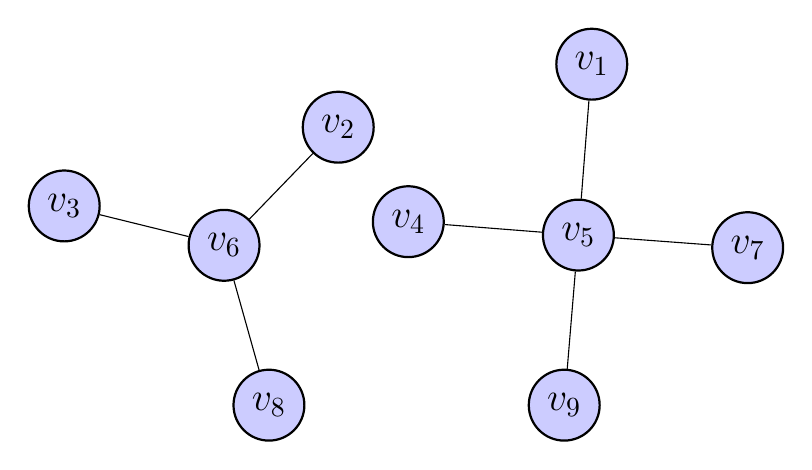
\begin{tikzpicture}[
  scale=1,
  vnode/.style={circle, fill=blue!20, draw=black, thick, minimum size=9mm, inner sep=0pt, font=\Large}
]
  % Vértices
  \node[vnode] (v1) at (7.05, 4.75) {$v_1$};
  \node[vnode] (v2) at (3.83, 3.95) {$v_2$};
  \node[vnode] (v3) at (0.35, 2.95) {$v_3$};
  \node[vnode] (v4) at (4.72, 2.75) {$v_4$};
  \node[vnode] (v5) at (6.88, 2.58) {$v_5$};
  \node[vnode] (v6) at (2.38, 2.45) {$v_6$};
  \node[vnode] (v7) at (9.03, 2.42) {$v_7$};
  \node[vnode] (v8) at (2.95, 0.42) {$v_8$};
  \node[vnode] (v9) at (6.70, 0.42) {$v_9$};

  % Aristas
  \foreach \from/\to in {v1/v5, v2/v6, v3/v6, v4/v5, v5/v7, v5/v9, v6/v8}
    \draw (\from) -- (\to);
\end{tikzpicture}
}}}$
            &
            $\vcenter{\hbox{$\displaystyle \begin{pmatrix}
         0 & 0 & 0 & 0 & 1 & 0 & 0 & 0 & 0 \\
         0 & 0 & 0 & 0 & 0 & 1 & 0 & 0 & 0 \\
         0 & 0 & 0 & 0 & 0 & 1 & 0 & 0 & 0 \\
         0 & 0 & 0 & 0 & 1 & 0 & 0 & 0 & 0 \\
         1 & 0 & 0 & 1 & 0 & 0 & 1 & 0 & 1 \\
         0 & 1 & 1 & 0 & 0 & 0 & 0 & 1 & 0 \\
         0 & 0 & 0 & 0 & 1 & 0 & 0 & 0 & 0 \\
         0 & 0 & 0 & 0 & 0 & 1 & 0 & 0 & 0 \\
         0 & 0 & 0 & 0 & 1 & 0 & 0 & 0 & 0
      \end{pmatrix}$}}$ \\
            \noalign{\vspace{6pt}}
         \end{tabular}%
      } \\
      \hline
      \multicolumn{3}{c}{\textbf{Topología de adyacencia}} \\
      \hline
      Abiertos subbásicos & Vecindades mínimas & Topología \\
      \hline
         ${A_{v_1}=\{v_5\}}$\par
         ${A_{v_2}=\{v_6\}}$\par
         ${A_{v_3}=\{v_6\}}$\par
         ${A_{v_4}=\{v_5\}}$\par
         ${A_{v_5}=\{v_1,v_4,v_7,v_9\}}$\par
         ${A_{v_6}=\{v_2,v_3,v_8\}}$\par
         ${A_{v_7}=\{v_5\}}$\par
         ${A_{v_8}=\{v_6\}}$\par
         ${A_{v_9}=\{v_5\}}$
      &
         ${U_{v_1}=\{v_1,v_4,v_7,v_9\}}$\par
         ${U_{v_2}=\{v_2,v_3,v_8\}}$\par
         ${U_{v_3}=\{v_2,v_3,v_8\}}$\par
         ${U_{v_4}=\{v_1,v_4,v_7,v_9\}}$\par
         ${U_{v_5}=\{v_5\}}$\par
         ${U_{v_6}=\{v_6\}}$\par
         ${U_{v_7}=\{v_1,v_4,v_7,v_9\}}$\par
         ${U_{v_8}=\{v_2,v_3,v_8\}}$\par
         ${U_{v_9}=\{v_1,v_4,v_7,v_9\}}$
      &
         $\{\emptyset,$ $\{v_5\},$ $\{v_6\},$ $\{v_5,v_6\},$ $\{v_2,v_3,v_8\},$ $\{v_1,v_4,v_7,v_9\},$ $\{v_2,v_3,v_5,v_8\},$ $\{v_2,v_3,v_6,v_8\},$ $\{v_1,v_4,v_5,v_7,v_9\},$ $\{v_1,v_4,v_6,v_7,v_9\},$ $\{v_2,v_3,v_5,v_6,v_8\},$ $\{v_1,\allowbreak v_4,\allowbreak v_5,\allowbreak v_6,\allowbreak v_7,\allowbreak v_9\},$ $\{v_1,\allowbreak v_2,\allowbreak v_3,\allowbreak v_4,\allowbreak v_7,\allowbreak v_8,\allowbreak v_9\},$ $\{v_1,\allowbreak v_2,\allowbreak v_3,\allowbreak v_4,\allowbreak v_5,\allowbreak v_7,\allowbreak v_8,\allowbreak v_9\},$ $\{v_1,\allowbreak v_2,\allowbreak v_3,\allowbreak v_4,\allowbreak v_6,\allowbreak v_7,\allowbreak v_8,\allowbreak v_9\},$ $\{v_1,\allowbreak v_2,\allowbreak v_3,\allowbreak v_4,\allowbreak v_5,\allowbreak v_6,\allowbreak v_7,\allowbreak v_8,\allowbreak v_9\}\}$ \\[6pt]
      \hline
      \multicolumn{3}{c}{\textbf{Topología de incidencia}} \\
      \hline
      Abiertos subbásicos & Vecindades mínimas & Topología \\
      \hline
         ${e_{1}=\{v_1,v_5\}}$\par
         ${e_{2}=\{v_2,v_6\}}$\par
         ${e_{3}=\{v_3,v_6\}}$\par
         ${e_{4}=\{v_4,v_5\}}$\par
         ${e_{5}=\{v_5,v_7\}}$\par
         ${e_{6}=\{v_5,v_9\}}$\par
         ${e_{7}=\{v_6,v_8\}}$
      &
         ${U_{v_1}=\{v_1,v_5\}}$\par
         ${U_{v_2}=\{v_2,v_6\}}$\par
         ${U_{v_3}=\{v_3,v_6\}}$\par
         ${U_{v_4}=\{v_4,v_5\}}$\par
         ${U_{v_5}=\{v_5\}}$\par
         ${U_{v_6}=\{v_6\}}$\par
         ${U_{v_7}=\{v_5,v_7\}}$\par
         ${U_{v_8}=\{v_6,v_8\}}$\par
         ${U_{v_9}=\{v_5,v_9\}}$
      &
         No discreta, con 153 abiertos \\[6pt]
      \hline
   \end{tabular}
   \caption{Topologías de adyacencia e incidencia de $G_8$}
   \label{tab:topologias_G_8}
\end{table}

\clearpage
\begin{table}[p]
   \centering
   \footnotesize
   \renewcommand{\arraystretch}{1.15}
   \begin{tabular}{@{}>{\centering\arraybackslash}m{0.3033\textwidth}>{\centering\arraybackslash}m{0.3033\textwidth}>{\centering\arraybackslash}m{0.3033\textwidth}@{}}
      \hline
      \multicolumn{3}{@{}c@{}}{%
         \begin{tabular}{@{}>{\centering\arraybackslash}m{\dimexpr0.455\textwidth+\tabcolsep\relax}>{\centering\arraybackslash}m{\dimexpr0.455\textwidth+\tabcolsep\relax}@{}}
            $G_9$ & Matriz de adyacencia \\
            \hline
            \noalign{\vspace{6pt}}
            \rule{0pt}{0pt}$\vcenter{\hbox{\resizebox{0.25\textwidth}{!}{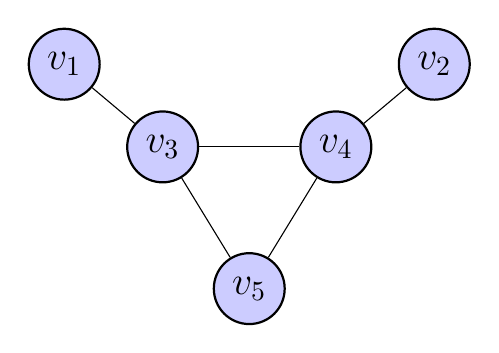
\begin{tikzpicture}[
  scale=1,
  vnode/.style={circle, fill=blue!20, draw=black, thick, minimum size=9mm, inner sep=0pt, font=\Large}
]
  % Vértices
  \node[vnode] (v1) at (0, 3.1) {$v_1$};
  \node[vnode] (v2) at (4.7, 3.1) {$v_2$};
  \node[vnode] (v3) at (1.25, 2.05) {$v_3$};
  \node[vnode] (v4) at (3.45, 2.05) {$v_4$};
  \node[vnode] (v5) at (2.35, 0.25) {$v_5$};

  % Aristas
  \foreach \from/\to in {v1/v3, v2/v4, v3/v4, v3/v5, v4/v5}
    \draw (\from) -- (\to);
\end{tikzpicture}
}}}$
            &
            $\vcenter{\hbox{$\displaystyle \begin{pmatrix}
         0 & 0 & 1 & 0 & 0 \\
         0 & 0 & 0 & 1 & 0 \\
         1 & 0 & 0 & 1 & 1 \\
         0 & 1 & 1 & 0 & 1 \\
         0 & 0 & 1 & 1 & 0
      \end{pmatrix}$}}$ \\
            \noalign{\vspace{6pt}}
         \end{tabular}%
      } \\
      \hline
      \multicolumn{3}{c}{\textbf{Topología de adyacencia}} \\
      \hline
      Abiertos subbásicos & Vecindades mínimas & Topología \\
      \hline
         ${A_{v_1}=\{v_3\}}$\par
         ${A_{v_2}=\{v_4\}}$\par
         ${A_{v_3}=\{v_1,v_4,v_5\}}$\par
         ${A_{v_4}=\{v_2,v_3,v_5\}}$\par
         ${A_{v_5}=\{v_3,v_4\}}$
      &
         ${U_{v_1}=\{v_1,v_4,v_5\}}$\par
         ${U_{v_2}=\{v_2,v_3,v_5\}}$\par
         ${U_{v_3}=\{v_3\}}$\par
         ${U_{v_4}=\{v_4\}}$\par
         ${U_{v_5}=\{v_5\}}$
      &
         $\{\emptyset,$ $\{v_3\},$ $\{v_4\},$ $\{v_5\},$ $\{v_3,v_4\},$ $\{v_3,v_5\},$ $\{v_4,v_5\},$ $\{v_1,v_4,v_5\},$ $\{v_2,v_3,v_5\},$ $\{v_3,v_4,v_5\},$ $\{v_1,v_3,v_4,v_5\},$ $\{v_2,v_3,v_4,v_5\},$ $\{v_1,v_2,v_3,v_4,v_5\}\}$ \\[6pt]
      \hline
      \multicolumn{3}{c}{\textbf{Topología de incidencia}} \\
      \hline
      Abiertos subbásicos & Vecindades mínimas & Topología \\
      \hline
         ${e_{1}=\{v_1,v_3\}}$\par
         ${e_{2}=\{v_2,v_4\}}$\par
         ${e_{3}=\{v_3,v_4\}}$\par
         ${e_{4}=\{v_3,v_5\}}$\par
         ${e_{5}=\{v_4,v_5\}}$
      &
         ${U_{v_1}=\{v_1,v_3\}}$\par
         ${U_{v_2}=\{v_2,v_4\}}$\par
         ${U_{v_3}=\{v_3\}}$\par
         ${U_{v_4}=\{v_4\}}$\par
         ${U_{v_5}=\{v_5\}}$
      &
         $\{\emptyset,$ $\{v_3\},$ $\{v_4\},$ $\{v_5\},$ $\{v_1,v_3\},$ $\{v_2,v_4\},$ $\{v_3,v_4\},$ $\{v_3,v_5\},$ $\{v_4,v_5\},$ $\{v_1,v_3,v_4\},$ $\{v_1,v_3,v_5\},$ $\{v_2,v_3,v_4\},$ $\{v_2,v_4,v_5\},$ $\{v_3,v_4,v_5\},$ $\{v_1,v_2,v_3,v_4\},$ $\{v_1,v_3,v_4,v_5\},$ $\{v_2,v_3,v_4,v_5\},$ $\{v_1,v_2,v_3,v_4,v_5\}\}$ \\[6pt]
      \hline
   \end{tabular}
   \caption{Topologías de adyacencia e incidencia de $G_9$}
   \label{tab:topologias_G_9}

   \vspace{2em}
   \begin{minipage}{\textwidth}
      \normalsize
      El grafo $G_9$ es conocido como \textit{grafo toro}.
   \end{minipage}
\end{table}

